\documentclass[MS, xcolor=dvipsnames]{wfuthesis}
\usepackage{mathtools,amsthm,amssymb,mathrsfs}
\usepackage{graphicx}
\usepackage{xcolor}
\usepackage{enumitem}
\usepackage{pdfpages}

% \usepackage[backend=biber]{biblatex}
% \addbibresource{bibliography.bib}
\usepackage[pdfpagelabels,draft,implicit=false]{hyperref}
\urlstyle{same}
% \usepackage{soul}
% \usepackage{float}
% \usepackage{enumerate}
% \usepackage{multicol}
% \usepackage{tikz}
% \usetikzlibrary{matrix,arrows}
\usepackage[all]{xy}
% \usepackage{tikz-cd}
% \tikzcdset{every arrow/.append style = -{Latex[width=4pt,length=10pt]}}
\usepackage[defaultmono]{droidsansmono}
\usepackage{listings}
% \lstset{basicstyle=\xpt\droidsansmono}
% \usepackage{fontspec}
% \usepackage{setspace}
% \setmainfont{Times New Roman}
% \usepackage{derivative}
% \usepackage{fancyvrb}
% \renewcommand{\theFancyVerbLine}{\textsuperscript{\arabic{FancyVerbLine}}}
% \usepackage{multirow}
% \usepackage{dsfont}
\usepackage{indentfirst}
% \usepackage{blindtext}
\usepackage{lipsum}

\definecolor{codegreen}{rgb}{0,0.6,0}
\definecolor{codegray}{rgb}{0.5,0.5,0.5}
\definecolor{codepurple}{rgb}{0.58,0,0.82}
\definecolor{backcolour}{rgb}{0.95,0.95,0.92}

\lstset{escapechar=\&,
        basicstyle=\xpt\droidsansmono,
        breaklines=true,
        showstringspaces=false,
        backgroundcolor=\color{backcolour}}
        % commentstyle=\color{codegreen},
        % keywordstyle=\color{blue},
        % stringstyle=\color{codepurple}}

% \DeclarePairedDelimiter{\ceil}{\lceil}{\rceil}
% \DeclarePairedDelimiter{\floor}{\lfloor}{\rfloor}
% \def\bA{\mathbb{A}}
% \def\cB{\mathcal{B}}
\def\bC{\mathbb{C}}
\def\sC{\mathsf{C}}
\def\sD{\mathsf{D}}
\def\sE{\mathsf{E}}
\def\bF{\mathbb{F}}
\def\cF{\mathcal{F}}
\def\cG{\mathcal{G}}
% \def\bH{\mathbb{H}}
% \def\bI{\mathbb{I}}
% \def\cL{\mathcal{L}}
% \def\cM{\mathcal{M}}
\def\bN{\mathbb{N}}
\def\cP{\mathcal{P}}
\def\bQ{\mathbb{Q}}
\def\bR{\mathbb{R}}
\def\cT{\mathcal{T}}
\def\Hask{\mathsf{Hask}}
% \def\cU{\mathcal{U}}
% \def\bV{\mathbb{V}}
\def\bZ{\mathbb{Z}}
% \def\bk{\bk}
\def\sbs{\subseteq}
\def\sps{\supseteq}

% \newcommand{\upperset}[2]{\:
% \underset{
%   \text{\raisebox{1.2ex}{\smash{\scalebox{0.8}{$#1$}}}}
% }{
%   \text{\raisebox{0.2ex}{\smash{$#2$}}}
% }
% \:}
% \def\opset{\upperset{\text{\tiny{open}}} \subset}
% \def\clset{\upperset{\text{\tiny{closed}}} \subset}

% \DeclareMathOperator{\Aut}{Aut}
% \DeclareMathOperator{\Dim}{Dim}
% \DeclareMathOperator{\ev}{ev}
\DeclareMathOperator{\gb}{gb}
% \DeclareMathOperator{\GL}{GL}
\DeclareMathOperator{\Hom}{Hom}
\DeclareMathOperator{\id}{id}
\DeclareMathOperator{\im}{im}
\DeclareMathOperator{\lcm}{lcm}
% \DeclareMathOperator{\Mat}{Mat}
% \DeclareMathOperator{\nullsp}{null}
% \DeclareMathOperator{\range}{range}
% \DeclareMathOperator{\SL}{SL}
\DeclareMathOperator{\Span}{span}
\newcommand{\LT}{\ensuremath{\text{\sc lt}}}
\newcommand{\LM}{\ensuremath{\text{\sc lm}}}
\newcommand{\LC}{\ensuremath{\text{\sc lc}}}
\DeclareMathOperator{\multideg}{multideg}
\def\and{\text{ and }}

\newtheorem{theorem}{Theorem}
\newtheorem{lemma}[theorem]{Lemma}
\newtheorem{observation}[theorem]{Observation}
\newtheorem{proposition}[theorem]{Proposition}
\newtheorem{corollary}[theorem]{Corollary}
\theoremstyle{definition}
\newtheorem{definition}[theorem]{Definition}
\newtheorem{example}[theorem]{Example}

% \def\e{\epsilon}
% \def\d{\delta}
\def\p{\varphi}

\begin{document}
\title{A Functional Computer Algebra System for Polynomials}
\author{Thomas Meek}
\department{Mathematics}

\advisor{W. Frank Moore, Ph.D.}
\chairperson{Ellen Kirkman, Ph.D.}
\member{William Turkett, Ph.D.}

\date{May, 2023}

\maketitle

\clearpage

\acknowledgments 

\lipsum[1]

\tableofcontents

\abstract

The \lstinline{polynomial-algorithms} package is a computer algebra system written in Haskell. This package implements a Polynomial type for use in several algorithms including a recursive version of Buchberger's algorithm for finding the reduced Gr\"obner basis of a polynomial ideal. As it is written in Haskell, the \lstinline{polynomial-algorithms} package naturally uses a purely functional design philosophy. We will contrast this with imperative approaches using more traditional languages. 

\chapters

\chapter{Introduction}
The theory of polynomials is a well-studied field of mathematics, rich with results which provide tools for mathematicians in various areas. Polynomial functions are among the simplest continuous functions to work with analytically or algebraically. Computationally, they are unquestionably the most important class of functions. It is then imperative to have a robust collection of software that can assist the mathematicians who study them. Many tools currently exist for this purpose, from dedicated high-level languages like Macaulay2 and Singular to libraries for general purpose languages like SageMath and SimPy. These software collections are referred to as \textit{computer algebra systems} or CAS's and while most have capabilities beyond polynomial manipulation, it is this feature that is the focus here. \par 
The implementation of these tools varies greatly. The Macaulay2 engine is written in C++ \cite{M2} while SageMath is built with Python \cite{SageMath}, which in turn often calls C. Their respective interfaces often use a mixture of procedural, object-oriented, functional, and declarative design. This certainly makes sense in the case of SageMath as Python itself hybridizes these approaches. If a CAS is a package for a general purpose language like Python, it should obey the design principles of that language. For dedicated CAS's like Macaulay2 though, this design choice bears consideration. There is a tendency in modern languages to incorporate features which favor a variety of paradigms. The popularity of hybrid languages like Python and JavaScript has encouraged most newer languages like Rust and Go to follow in their footsteps. There are good reasons for this, however there are also benefits to sticking to a single paradigm. \par 
It is true that these paradigms are more a philosophical way of approaching software design than a well-defined feature of a language and given that, no language can be said to be strictly single-paradigm. It is clear however that certain languages lend themselves to being more compatible with one paradigm than others. For example, Java is generally seen as a paragon of object-oriented programming. Every module contains exactly one class (with potentially many subclasses). Even the drivers are classes and must be instantiated before any program can be executed. One can use Java in a functional way, but doing so defeats the purpose of using Java. This is in contrast to a language like Python where it is difficult to escape the use of objects and classes, but higher order functions like folds and maps are used frequently, as are list comprehensions and other hallmarks of functional programming. At the same time, most programmers' first experience with Python is in writing plain procedural scripts. The freedom offered by such a language enables one to choose the most appropriate approach to the current task, but in doing so, it takes away the cohesiveness and predictability of a more \textit{pure} language like Java. \par 
Similarly to the way Java is considered a paragon of the object-oriented school, Haskell is often one of the first two languages people think of when one mentions functional programming, with the other of course being Lisp. The functional style offers many advantages over a procedural or object-oriented approach as evidenced in how much modern languages have borrowed from Haskell. Rust's type system strongly resembles that of Haskell \cite{Poss2014} and modern JavaScript libraries like React  leverage functional programming more than any other paradigm. \par 
Haskell and the functional programming style are particularly well-suited to mathematics. The notion of a `function' in procedural programming is a bit of a misnomer. Mathematically, a function $f$ is a domain $X$, a codomain $Y$, and some subset of $X \times Y$ called the graph of $f$. What is the domain of the \lstinline{print()} function in Python? What is its codomain? What is its graph? These inconsistencies vanish in Haskell. A Haskell function \textit{is} a mathematical function. For this reason, mathematicians often regard the functional paradigm as the natural choice for mathematical software. What better way to determine the injectivity of a function than with a function whose injectivity can be determined?! \par 
It is in this spirit that the \lstinline{polynomial-algorithms} package was written. Taking advantage of the benefits offered by Haskell (as well as a few language extensions), this package offers a Polynomial type that is itself built on Monomial and Coefficient types. Several algorithms, most notably a modified version of Buchberger's algorithm to find a reduced Gr\"obner basis for a list of polynomials, are featured in this software. In addition, its scalability and modularity should provide mathematicians with an invaluable tool when analyzing polynomials. %TODO: Summarize the contents of the thesis here

\chapter{Mathematical Background}
One thing that sets functional programming apart from imperative paradigms is its reliance on mathematics. Writing algorithms or any sufficiently complex code will always require some familiarity with mathematics, and the best and most efficient code is often written by programmers competent in mathematical reasoning. However, this quality is even more important when working in a language like Haskell. This fact may be seen just by reading documentation. A good technical writer will always write to their audience. If one is writing a UDP server in Java, it may be assumed that anyone maintaining that server will be familiar with terms like \textit{port}, \textit{buffer}, or \textit{packet}, so they may appear frequently in documentation. If one is writing an operating system in C, terms like \textit{fork} and \textit{process ID} are ubiquitous enough to appear in documentation without explanation. However, one is unlikely to encounter mentions of algebraic ring theory in the documentation for such projects. When using Haskell, this is quite common \cite{Prelude}. \par 
It is therefore imperative (pun intended) for a prospective Haskeller\footnote{The term \textit{Haskeller} refers to a regular user of Haskell.} to have a working knowledge of several areas of mathematics not usually necessary for writing programs in a procedural or object-oriented style. This is doubly important when using Haskell to write a CAS. The fact that the recommended backgrounds for the problem domain and the solution domain coincide is further evidence that Haskell is indeed a good fit for such a task. \par 
As any software engineer will tell you, having a firm understanding of mathematical logic can be helpful in writing and debugging code. Boolean algebra is essential for the standard control flow mechanisms used in all languages. De Morgan's laws and other properties of first order logic can assist in cleaning up messy functions. It is well-known that a familiarity with combinatorics and graph theory can be helpful for those writing abstract data types or analyzing networks, and linear algebra and multivariate calculus are essential for working with 3D graphics. However, abstract algebra and category theory are rarely covered in the standard curriculum for a computer science degree. \par 
When using Haskell, a working knowledge of algebraic group theory and ring theory, while not strictly necessary, can provide useful insight into why certain typeclasses and functions behave the way they do. When writing a CAS, this recommendation is upgraded to a strict requirement. Even more central in the design of Haskell and other functionally-minded languages is the presence of the ever-intimidating category theory. Even by theoretical mathematicians, this subject is often referred to as \textit{abstract nonsense} \cite{Saunders1997}. Having a reputation as being among the most abstruse of mathematical topics, the mere fact that something as concrete and useful as writing software could employ such a concept is itself remarkable. \par 
Using such a mathematically inclined language to implement a CAS is clearly an endeavour that requires a thorough understanding of the mathematics at play. Of particular importance is the theory of polynomials. 

\section{Polynomials}
Polynomials in a single variable with real coefficients are a familiar object of study, not only to professional mathematicians, but to anyone who has taken a high school math class. They are easy to understand and work with. Finding their roots, taking their derivatives, and analyzing their graphs are among the easier tasks a mathematician will attempt. We even estimate arbitrary analytic functions as polynomials via Taylor's theorem. Many of the algorithms that form the backbone of low-level software are based on this idea. It should come as no surprise then that generalizing these familiar objects is a popular practice. Using fields other than $\bR$ is a natural first step. In fact, when using an algebraically closed field like $\bC$, polynomials behave even more nicely than they did over $\bR$ as we don't have to wonder how many roots a degree $n$ polynomial may have; the answer is always $n$ (up to multiplicity). \par 
The next natural generalization is to allow for multiple (though still finitely many) variables. This generalization does introduce some complexity. For one thing, the idea of ordering the terms, which was taken for granted in the single variable case, now becomes a nontrivial discussion. The tools from multivariate calculus can be helpful in understanding the analytic nature of multivariate polynomials, while an introductory course in abstract algebra or algebraic geometry often addresses the more algebraic concerns by introducing term orders, algorithms, and the relationship between the ideals containing these objects and the affine varieties they generate. 

\subsection{Monomials}
There are two competing ways to view a polynomial. The first is as a function from some ring into itself. It is this view that is usually encountered first, and for most analytic purposes, this is sufficient. The other way is as a formal linear combination of indeterminates. This is the view that we prefer in this discussion. These indeterminates comprise a free monoid\footnote{Recall that a monoid is a set with an associative binary operation and an identity element. Being free means there are no unforced relationships between elements. For example, $x \ne y^n$ for any $n$.}, and (at least for now) we may assume the monoidal operation to be commutative. We use the term \textit{monomial} when referring to elements of a free monoid in the context of polynomials. \par 
In this view, the phrase \textit{polynomial in n variables} really means a linear combination of monomials drawn from a free monoid with $n$ distinct generators. Each generator is called a variable. When dealing with polynomials in a single variable, we usually use the symbol $x$ to refer to the generator of this monoid. So the polynomial $f$ defined as 
\[ f(x) = x^2-8x+15 \]
is a formal linear combination of the monomials $x^2$, $x$, and $1$ taken from the free monoid $\langle x \rangle$ with weights $1$,$-8$, and $15$. In the case of a three variable polynomial, the monoid used is generated by three elements. Here, there are two competing notational conventions. The first is to denote the generators as $x$, $y$, and $z$. The second is to denote the generators as $x_1$, $x_2$, and $x_3$. The former is often more readable, but the latter more easily generalizes to $n$ variables. \par 
This viewpoint of polynomials as a formal combination of monomials rather than a function may be summed up in the following few definitions. Note that these and the rest of the definitions in this section are courtesy of Cox, Little and O'Shea \cite{Cox2015}: 
\begin{definition}
  A \textbf{monomial} in $x_1,\dots,x_n$ is a product of the form 
  \[ x_1^{\alpha_1} \cdot x_2^{\alpha_2} \cdots x_n^{\alpha_n}, \]
  where all of the exponents $\alpha_1,\dots,\alpha_n$ are nonnegative integers. The \textbf{multidegree} of this monomial is the $n$-tuple $(\alpha_1,\alpha_2,\dots) \in \bZ_{\ge0}^n$. The \textbf{total degree} of this monomial is the sum $\alpha_1 + \dots + \alpha_n$.
\end{definition}
We can simplify the notation for monomials as follows: let $\alpha = (\alpha_1,\dots,\alpha_n)$ be an $n$-tuple of nonnegative integers. Then we set
\[ x^\alpha = x_1^{\alpha_1} \cdot x_2^{\alpha_2} \cdots x_n^{\alpha_n}. \]
When $\alpha=(0,\dots,0)$, note that $x^\alpha=1$. We also let $|\alpha| = \alpha_1 + \dots + \alpha_n$ denote the total degree of the monomial $x^\alpha$.
\begin{definition}
  A \textbf{polynomial} $f$ in $x_1,\dots,x_n$ with coefficients in a field $k$ is a finite linear combination (with coefficients in $k$) of monomials. We will write a polynomial $f$ in the form
  \[ f = \sum_\alpha a_\alpha x^\alpha,\quad a_\alpha \in k, \]
  where the sum is over a finite number of $n$-tuples $\alpha = (\alpha_1,\dots,\alpha_n)$. The set of all polynomials in $x_1,\dots,x_n$ with coefficients in $k$ is denoted $k[x_1,\dots,x_n]$. 
\end{definition}
\begin{definition}
  Let $f = \sum_\alpha a_\alpha x^\alpha$ be a polynomial in $k[x_1,\dots,x_n]$. 
  \begin{enumerate}[label=(\roman*)]
    \item We call $a_\alpha$ the \textbf{coefficient} of the monomial $x^\alpha$. 
    \item If $a_\alpha\ne0$, then we call $a_\alpha x^\alpha$ a \textbf{term} of $f$. 
    \item The \textbf{total degree} of $f \ne 0$, denoted $\deg(f)$, is the maximum $|\alpha|$ such that the coefficient $a_\alpha$ is nonzero. The total degree of the zero polynomial is undefined.
  \end{enumerate}
\end{definition}
One observation is that the set $k[x_1,\dots,x_n]$ forms a ring under the standard polynomial addition and multiplication operations. In the case where $n=1$, the ring $k[x]$ contains the familiar polynomials in a single variable. An important question that often arises when working with polynomials in more than one variable is how to define the leading term. Given a nonzero polynomial $f \in k[x]$, let
\[ f = c_0x^m + c_1x^{m-1} + \dots + c_m, \]
where $c_i \in k$ and $c_0 \ne 0$ (thus $\deg(f)=m$). Then we say that $c_0x^m$ is the \textbf{leading term} of $f$ and write $\LT(f)=c_0x^m$. The leading term of a polynomial is a surprisingly essential characteristic. For example, when executing single variable polynomial long division, the first step is to make sure the polynomial is expressed with its leading term first, and at each subsequent step, that must remain the case; but what about when there are multiple variables? Given the polynomial $g \in k[x,y,z]$ defined as 
\[ g = xy^2z^3 + x^5 + x^3y^2z, \]
what is the leading term of $g$? We will have to be careful about how we define the leading term in this case, as there is not just one obvious way. \par 
This leads us to a discussion of \textit{monomial orderings}. There are uncountably many ways to order the monomials in a free monoid, but the majority of them will not be compatible with polynomial multiplication in the way we would like. The orderings that we may use must satisfy a few special properties, espoused in the following definition \cite{Cox2015}:
\begin{definition}
  A \textbf{monomial ordering} on $k[x_1,\dots,x_n]$ is a relation $>$ on the set of monomials $x^\alpha$, $\alpha \in \bZ_{\ge0}^n$ satisfying:
  \begin{enumerate}[label=(\roman*)]
    \item $>$ is a total ordering\footnote{Recall $>$ is a total ordering if for all $\alpha,\beta$ exactly one of $x^\alpha > x^\beta$, $x^\alpha = x^\beta$, or $x^\beta > x^\alpha$ is true.}. 
    \item If $x^\alpha > x^\beta$ and $\gamma \in \bZ_{\ge0}^n$, then $x^\alpha x^\gamma > x^\beta x^\gamma$. 
    \item $>$ is a well-ordering. 
  \end{enumerate}
\end{definition}
It turns out that the third condition above is equivalent to two other statements that are easier to work with. 
\begin{theorem}
  Let $X$ be a commutative free monoid and suppose the first two conditions in the definition above are satisfied. Then the following are equivalent: 
  \begin{enumerate}
    \item $>$ is a well-ordering on $X$. 
    \item Every strictly decreasing sequence in $X$ eventually terminates. 
    \item $x^\alpha\ge1$ for all $\alpha \in \bZ_{\ge0}^n$. 
  \end{enumerate}
\end{theorem}
For a proof of this theorem, see Cox, Little and O'Shea \cite{Cox2015}. This allows us to show that certain algorithms terminate by showing that some term strictly decreases at each step of the algorithm. \par 
Now that we have a well-defined way to order monomials, we are ready to define a few more terms.
\begin{definition}
  Let $f = \sum_\alpha a_\alpha x^\alpha$ be a nonzero polynomial in $k[x_1,\dots,x_n]$ and let $>$ be a monomial order.
  \begin{enumerate}[label=(\roman*)]
    \item The \textbf{multidegree} of $f$ is 
    \[ \multideg(f) = \max(\alpha \in \bZ_{\ge0}^n \mid a_\alpha \ne 0) \]
    (the maximum is taken with respect to $>$).
    \item The \textbf{leading coefficient} of $f$ is
    \[ \LC(f) = a_{\multideg(f)} \in k. \]
    \item The \textbf{leading monomial} of $f$ is
    \[ \LM(f) = x^{\multideg(f)}. \]
    \item The \textbf{leading term} of $f$ is
    \[ \LT(f) = \LC(f) \cdot \LM(f). \]
  \end{enumerate}
\end{definition}
There are many monomial orderings that are used frequently in research, however we will limit our attention to three specific examples. The first such example is perhaps the most intuitive. 
\begin{definition}[\bf Lexicographic Order]
  Let $\alpha = (\alpha_1, \dots, \alpha_n)$ and $\beta = (\beta_1,\dots,\beta_n)$ be in $\bZ_{\ge0}^n$. We say $x^\alpha >_{Lex} x^\beta$ if the leftmost nonzero entry of the vector difference $\alpha - \beta \in \bZ^n$ is positive. 
\end{definition}
The Lexicographic order is the order used in most dictionaries. We begin with an ordering of the variables. The greater monomial is the one with the larger exponent in the first variable. If those exponents are the same, we instead calculate the Lexicographic order without the highest variable. In our previous example, $g = xy^2z^3 + x^5 + x^3y^2z$, we see that the lead term under the Lexicographic order where $x>y>z$ is $\LT(g)=x^5$. By convention, when denoting variables with subscripts, we take $x_1 > x_2 > x_3 > \dots$. \par 
Our next monomial ordering is built out of the Lexicographic order. 
\begin{definition}[\bf Graded Lex Order]
  Let $\alpha,\beta \in \bZ_{\ge0}^n$. We say $x^\alpha >_{GLex} x^\beta$ if $|\alpha| > |\beta|$ or $|\alpha|=|\beta|$ and $x^\alpha >_{Lex} x^\beta$. 
\end{definition}
This means that the Graded Lex order first orders by total degree, but breaks ties with the Lexicographic order. In our running example using the Graded Lex order, we see that $\LT(g)=x^3y^2z$. \par 
Our third and final monomial ordering is less intuitive than the previous two.
\begin{definition}[\bf Graded Reverse Lex Order]
  Let $\alpha,\beta \in \bZ_{\ge0}^n$. We say $x^\alpha >_{GRevLex} x^\beta$ if $|\alpha| > |\beta|$ or $|\alpha|=|\beta|$ and the rightmost nonzero entry of $\alpha - \beta \in \bZ^n$ is negative. 
\end{definition}
Here, we are still ordering first by total degree, but we break ties in a manner that is in a way the \emph{double reversal} of Lexicographic order. Using the Graded Reverse Lex order, the lead term of $g$ is $xy^2z^3$. As unintuitive as the Graded Reverse Lex order may seem, it turns out that this ordering is often the most efficient in many algorithms, including some we will explore here. 

\subsection{Ideals}
In general, when $R$ is a commutative ring, a subring $I$ (not necessarily with identity) is an ideal if $ra \in I$ for all $r \in R$ and $a \in I$. For the polynomial ring $k[x_1,\dots,x_n]$ this means that an ideal is a nonempty subset closed under subtraction which absorbs polynomials by multiplication. For example, let $S \sbs k[x]$ be the set of polynomials with no constant or linear terms, so that $0 \in S$ and for any nonzero $f \in S$, the lowest degree term of $f$ has degree at least two. Then $S$ is easily seen to be an ideal of $k[x]$. In fact, $S$ is what is known as a \textit{principal ideal} because $S$ is \textit{generated} by a single polynomial, namely the polynomial $x^2$. This means that any polynomial in $S$ may be formed by multiplying $x^2$ by some polynomial in $k[x]$. More generally, an ideal $I \in k[x_1,\dots,x_n]$ is said to be generated by a set $B$ of polynomials if every $f \in I$ may be expressed as $f = b_1f_1 + \dots + b_tf_t$ for some $b_1,\dots,b_t \in B$ and some $f_1,\dots,f_t \in k[x_1,\dots,x_n]$. In this case, we write $I = \langle B \rangle$. In our example above, we would write $S = \langle x^2 \rangle$. It turns out that \textit{every} ideal in $k[x]$ is generated by a single polynomial, making this ring quite important in algebra and number theory. When dealing with multiple variables, we have no such luck. There is no single polynomial that generates the ideal $\langle x,y \rangle \in k[x,y,z]$. However, it is true that every polynomial ideal is generated by \textit{some} set since an ideal will generate itself. What is more impressive and not quite as obvious is the fact that every polynomial ideal is generated by some \textit{finite} set. This result was first proved by David Hilbert in 1890 and is known as \textit{Hilbert's Basis Theorem} \cite{Hilbert1890}. \par 
Combining our notion of the leading term of a polynomial with ideals in a polynomial ring leads us to the following definition.
\begin{definition}
  Let $I \sbs k[x_1,\dots,x_n]$ be an ideal other than $\{0\}$, and fix a monomial ordering on $k[x_1,\dots,x_n]$. Then: 
  \begin{enumerate}[label=(\roman*)]
    \item We denote by $\LT(I)$ the set of leading terms of nonzero elements of $I$. Thus,
    \[ \LT(I) = \{ cx^\alpha \mid \text{ there exists } f \in I \setminus \{0\} \text{ with } \LT(f) = cx^\alpha \}. \]
    \item We denote by $\langle \LT(I) \rangle$ the ideal generated by the elements of $\LT(I)$. 
  \end{enumerate}
\end{definition}
If $I \sbs k[x_1,\dots,x_n]$ is an ideal then by Hilbert's Basis Theorem, there is some finite set of polynomials $\{ b_1,\dots,b_t \} \sbs k[x_1,\dots,x_n]$ such that $I = \langle b_1,\dots,b_t \rangle$. Since $b_1,\dots,b_t \in I$, it is clear that $\langle \LT(b_1), \dots, \LT(b_t) \rangle \sbs \langle \LT(I) \rangle$. However, this containment may be proper. Only in a very special case do we achieve equality of these two sets. 
\begin{example}
  Let $I = \langle f_1,f_2 \rangle \sbs \bQ[x,y]$, where $f_1=x^3-2xy$ and $f_2=x^2y-2y^2+x$, and use the Graded Reverse Lex order on monomials in $\bQ[x,y]$. Then 
  \[ x \cdot f_2 - y \cdot f_1 = x^2, \]
  so that $x^2 \in I$. Thus $x^2 = \LT(x^2) \in \langle \LT(I) \rangle$. However $x^2$ is not divisible by $\LT(f_1)$ or $\LT(f_2)$ so $x^2 \notin \langle \LT(f_1), \LT(f_2) \rangle$. 
\end{example}

\subsection{Gr\"obner bases}
We mentioned polynomial long division before when making the case for why a monomial ordering is necessary. Another challenge when working with multiple variables is that, even when we have the requisite ordering to preform long division, the quotient and remainder may depend on the order of the dividends. When dividing $f$ by the ordered list $(g_1,g_2,g_3)$, we may get a different result from when dividing $f$ by the ordered list $(g_2,g_3,g_1)$. While the quotient is unfortunately doomed to this fate, there is a way we may guarantee the uniqueness of at least the remainder. It turns out this uniqueness is crucial for many of the theorems and algorithms that mathematicians rely on. \par 
\begin{definition}
  Fix a monomial order on the polynomial ring $k[x_1,\dots,x_n]$. A finite subset $G = \{ g_1,\dots,g_t \}$ of an ideal $I \sbs k[x_1,\dots,x_n]$ different from $\{0\}$ is said to be a \textbf{Gr\"obner basis} if
  \[ \langle \LT(g_1), \dots, \LT(g_t) \rangle = \langle \LT(I) \rangle. \]
  Using the convention that $\langle \emptyset \rangle = {0}$, we define the empty set $\emptyset$ to be the Gr\"obner basis of the zero ideal $\{0\}$.
\end{definition}
Another way to state this definition is that the set $G = \{ g_1,\dots,g_t \}$ is a Gr\"obner basis for $I$ if the leading term of any element of $I$ is divisible by one of the $\LT(g_i)$. As one would expect from the terminology, a Gr\"obner basis is a generating set for the ideal $I$ in the definition above and it can be shown that every ideal has a Gr\"obner basis. This is lucky because much of modern polynomial theory and algebraic geometry depends on the existence of such a basis. This is partly because the Gr\"obner basis is the set we needed to guarantee uniqueness of the remainder in the division algorithm. \par 
Another feature of Gr\"obner bases is a solution to the so called \emph{ideal membership problem}. For a proof of the following theorem, see \cite{Cox2015}.
\begin{theorem}
  Let $G = \{ g_1,\dots,g_t \}$ be a Gr\"obner basis for an ideal $I \sbs k[x_1,\dots,x_n]$ and let $f \in k[x_1,\dots,x_n]$. Then $f \in I$ if and only if the remainder on division of $f$ by $G$ is zero. 
\end{theorem}
The remainder is sometimes called the \textbf{normal form} of $f$. We will use the following notation for the remainder.
\begin{definition}
  We will write $\overline f^{F}$ for the remainder on division of $f$ by the ordered $s$-tuple $F = (f_1,\dots,f_s)$. If $F$ is a Gr\"obner basis for $\langle f_1,\dots,f_s \rangle$, then we can regard $F$ as a set  (without any particular order). 
\end{definition}
One application of the division algorithm is Buchberger's algorithm for finding a Gr\"obner basis for the ideal $\langle f_1,\dots,f_t \rangle$. The idea behind this algorithm is to start with a list $(f_1,\dots,f_t)$, determine all polynomials in $\langle f_1,\dots,f_t \rangle$ that may have a lead term that isn't divisible by any of the $\LT(f_i)$, and add to the list the ones that aren't. To find a polynomial with lead term that isn't divisible by any of the $\LT(f_i)$, we need to construct a polynomial in our ideal that has a potentially different lead term from the generators. We do this by calculating \emph{$S$-polynomials}. The way we check if our set can generate this $S$-polynomial is via the division algorithm. 
\begin{definition}
  Let $f,g \in k[x_1,\dots,x_n]$ be nonzero polynomials. 
  \begin{itemize}
    \item If $\multideg(f) = \alpha$ and $\multideg(g) = \beta$, then let $\gamma  =(\gamma_1,\dots,\gamma_n)$, where $\gamma_i = \max(\alpha_i,\beta_i)$ for each $i$. We call $x^\gamma$ the \textbf{least common multiple} of $\LM(f)$ and $\LM(g)$, written $x^\gamma = \lcm(\LM(f),\LM(g))$. 
    \item The \textbf{$\mathbf S$-polynomial} of $f$ and $g$ is the combination 
    \[ S(f,g) = \frac{x^\gamma}{\LT(f)} \cdot f - \frac{x^\gamma}{\LT(g)} \cdot g. \]
  \end{itemize}
  (Note that we are inverting the leading coefficients here as well.)
\end{definition}
This definition leads to a crucial result in the theory of Gr\"obner bases.
\begin{theorem}[Buchberger's Criterion]
  Let $I$ be a polynomial ideal. Then a basis $G = \{g_1,\dots,g_t\}$ of $I$ is a Gr\"obner basis of $I$ if and only if for all pairs $i \ne j$, the remainder on division of $S(g_i,g_j)$ by $G$ (listed in some order) is zero.
\end{theorem}
Gr\"obner bases for ideals in polynomial rings were introduced by Bruno Buchberger in his PhD thesis \cite{Buchberger1965} and named by him in honor of Wolfgang Gr\"obner, Buchberger's thesis adviser. This construction sharply influenced the direction of computational algebra for the next half century. It is then no surprise that finding a Gr\"obner basis for a polynomial ideal in the most efficient way is a task of central importance in the field. Bruno Buchberger also developed the eponymous Buchberger's algorithm and since then, many tweaks and improvements have been made, but the basic logic of the algorithm remains largely unchanged. 

\section{Categories}
Over the last seventy-five years, the landscape of mathematics research has shifted in many ways. One of these ways is the ubiquity of categories in many mathematical fields. Modern mathematicians dealing with sheaves or tensors are more likely to use their categorical definitions than classical constructions. There are increasingly many attempts to introduce category theory to undergraduate mathematics students \cite{Aluffi2009}. Still, category theory has not shed its reputation for being overly abstract and useless outside of the purest of mathematical endeavors. To be fair, the first criticism is justified. Category theory is indeed abstract. Perhaps this is why the aforementioned attempts to introduce this theory to a less experienced audience have not yet become standard practice. The second criticism however is simply unfounded. \par 
Apart from providing more elegant solutions to mathematical problems found in other fields, and providing a unified framework with which to explore the relationships between otherwise unrelated disciplines, category theory does have actual applications outside of pure mathematics. For an example, one need look no further than the Haskell language. One of the most commonly used typeclasses is the Functor typeclass, which specifies a mechanism for \emph{mapping over} some structure. The idea of a functor is taken from category theory and is essential for writing high-quality software in the Haskell language. The remaining definitions in this chapter are largely taken from Emily Riehl's \textit{Category Theory in Context} \cite{Riehl2016}.
\begin{definition}
  A \textbf{category} $\sC$ is a collection of \textbf{objects} and \textbf{morphisms} such that: 
  \begin{itemize}
    \item Each morphism has specified \textbf{domain} and \textbf{codomain} objects. We denote the collection of morphisms with domain $a$ and codomain $b$ as $\Hom(a,b)$. If this collection is a set\footnote{The axioms of set theory may prevent this.}, we call $\Hom(a,b)$ the \textbf{hom set} of $(a,b)$. 
    \item Each object $x$ has a designated \textbf{identity morphism} $1_x \in \Hom(x,x)$. 
    \item If $f \in \Hom(a,b)$ and $g \in \Hom(b,c)$, then there is a morphism $gf \in \Hom(a,c)$. In this case, we say $f$ and $g$ are \textbf{composable} and $gf$ is their \textbf{composite}. 
  \end{itemize}
  This data is subject to the following two axioms: 
  \begin{itemize}
    \item For any $f \in \Hom(a,b)$, the composites $1_bf$ and $f1_a$ are both equal to $f$. 
    \item For any composable triple of morphisms $f,g,h$, the composites $h(gf)$ and $(hg)f$ are equal.
  \end{itemize}
\end{definition}
The prototypical example of a category is $\mathsf{Set}$ whose objects are sets and whose morphisms are the functions between those sets. In many categories, the morphisms are set-functions of some kind, but that is not always the case.
\begin{example}
  Recall that a poset is a set along with a relation that is reflexive, transitive, and antisymmetric. Let $(S,\le)$ be a poset. Then we may define a category $\mathsf S$ that has the elements of $S$ as its objects. If $a \le b$ then let $\Hom(a,b)$ be the singleton consisting of the element $(a,b) \in S \times S$. Otherwise, let $\Hom(a,b)=\emptyset$. Define the composition law as $(a,b)(b,c)=(a,c)$. As each hom set has at most a single element, there is only one choice for the identity morphism. \par
  If $(a,b)$ and $(b,c)$ both exist, then we must have that $a \le b \le c$, so since $\le$ is transitive, $(a,c)$ exists and so composition is well defined. Since $\le$ is reflexive, $(a,a) \in \Hom(a,a)$ and 
  \[ (a,a)(a,b) = (a,b) = (a,b)(b,b), \]
  so $(a,a)$ does serve as the identity on $a$. Also observe that 
  \[ ((a,b)(b,c))(c,d) = (a,c)(c,d) = (a,d) = (a,b)(b,d) = (a,b)((b,c)(c,d)), \]
  so composition is associative. This shows that $\mathsf S$ satisfies the axioms for a category. 
\end{example}
It is common in mathematics to introduce some kind of object that is only important because of the functions between objects of that kind. Linear algebra may be the study of vector spaces, but the important part is the linear maps. Topology may be concerned with open sets, but it is the continuous maps that topologists really care about. Group homomorphisms are in a sense are much more important than groups themselves. It is no different with categories. The interesting part is the maps between categories. The even more interesting part is the maps between those maps. 
\begin{definition}
  A \textbf{functor} $\cF: \sC \to \sD$ between categories $\sC$ and $\sD$ consists of the following data:
  \begin{itemize}
    \item An object $\cF x \in \sD$ for each object $x \in \sC$. 
    \item A morphism $\cF f \in \Hom(\cF a,\cF b)$ for each morphism $f \in \Hom(a,b)$. 
  \end{itemize}
  These assignments are required to satisfy the following axioms:
  \begin{itemize}
    \item For any composable pair of morphisms $f,g \in \sC$, $(\cF f) (\cF g) = \cF(gf)$. 
    \item For each object $x \in \sC$, $\cF(1_x) = 1_{\cF x}$. 
  \end{itemize}
  Given functors $\cF: \sC \to \sD$ and $\cG: \sD \to \sE$ it is easy to show that the composite $\cG \cF$ is a functor. 
\end{definition}
Given categories $\sC$ and $\sD$, we define $\sD^\sC$ to be the \textbf{functor category} from $\sC$ to $\sD$. The objects in $\sD^\sC$ are functors and the morphisms in $\sD^\sC$ are called \emph{natural transformations}. We call a functor between a category and itself an \textbf{endofunctor}. That is, an endofunctor on $\sC$ is an object in $\sC^\sC$. 
\begin{definition}
  Given functors $\cF, \cG: \sC \to \sD$, a \textbf{natural transformation} $\tau: \cF \Rightarrow \cG$ is a map from objects in $\sC$ to morphisms in $\sD$ that satisfies the following:
  \begin{itemize}
    \item If $x$ is an object in $\sC$, then $\tau_x$ is a morphism in $\Hom(\cF x, \cG x)$. 
    \item The following diagram commutes for all $a,b \in \sC$ and all $f \in \Hom(a,b)$. 
  \end{itemize}
  \[ \SelectTips{cm}{}\xymatrix@R+1pc@C+1pc{
      \cF a \ar[r]^{\tau_a} \ar[d]_{\cF f} & \cG a \ar[d]^{\cG f} \\ \cF b \ar[r]_{\tau_b} & \cG b%TODO: ask about a period here.
  } \]
\end{definition}
The idea of commuting diagrams is central to the study of category theory. It is a concise way of saying that any allowed composition of maps in the diagram will be equivalent if they share a domain and a codomain. A common categorical technique to prove theorems is called \emph{diagram chasing}. Diagram chasing involves finding equivalent map compositions. \par
\begin{definition}
  Given a natural transformation $\beta: \mathcal H \to \mathcal K$ and functors $\mathcal F$ and $\mathcal L$ as displayed in 
  \[ \SelectTips{cm}{}\xymatrix@C-1pc{
    \sC \ar[0,2]^{\cF} & & \sD \ar@/^1.5pc/[0,2]^{\mathcal H} \ar@/_1.5pc/[0,2]_{\mathcal K} & \Downarrow\beta & \mathsf E \ar[0,2]^{\mathcal L} & & \mathsf F
  } \]
  define a transformation $\mathcal L \beta \mathcal F: \mathcal L \mathcal H \mathcal F \Rightarrow \mathcal L \mathcal K \mathcal F$ by $(\mathcal L \beta \mathcal F)_x = \mathcal L \beta_{\mathcal F_x}$. This is the \textbf{whiskered composite} of $\beta$ with $\mathcal L$ and $\mathcal F$. It can be shown that $\mathcal L \beta \mathcal F$ is natural. If $\mathcal L$ is the identity functor, then $\mathcal L \beta \mathcal F = \beta \mathcal F$. If $\mathcal F$ is the identity functor, then  $\mathcal L \beta \mathcal F = \mathcal L \beta$. 
\end{definition}
We won't spend much time discussing the finer points of category theory. If teaching the fundamentals to a class of advanced undergraduate mathematics students over the course of a semester in their senior year is a bold undertaking, then explaining it in a single section of this document is a Kobayashi Maru\footnote{See \textit{Star Trek II: The Wrath of Khan} (1982).}. We do however need to address one more categorical construction before proceeding. 
\begin{definition}
  A \textbf{monad} on a category $\sC$ consists of 
  \begin{itemize}
    \item an endofunctor $\cT: \sC \to \sC$,
    \item a \textbf{unit} natural transformation $\eta: 1_\sC \Rightarrow \cT$, and 
    \item a \textbf{multiplication} natural transformation $\mu: \cT^2 \Rightarrow \cT$,
  \end{itemize}
  so that the following diagrams commute in $\sC^\sC$: 
\[ \SelectTips{cm}{}\xymatrix@R+1pc@C+1pc{
  \cT^3 \ar@{=>}[r]^{\cT\mu} \ar@{=>}[d]_{\mu \cT} & \cT^2 \ar@{=>}[d]^\mu \\ \cT^2 \ar@{=>}[r]_\mu & \cT
} \qquad\qquad \SelectTips{cm}{}\xymatrix@R+1pc@C+1pc{
  \cT \ar@{=>}[r]^{\eta \cT} \ar@{=>}[dr]_{1_\cT} & \cT^2 \ar@{=>}[d]^\mu & \cT \ar@{=>}[l]_{\cT\eta} \ar@{=>}[dl]^{1_\cT} \\ & \cT &
} \]
\end{definition}
In these diagrams, $\cT\eta,\eta\cT: T \Rightarrow T^2$ are defined as 
\[ (\cT\eta)_x = \cT(\eta_x) \qquad\and\qquad (\eta\cT)_x = \eta_{\cT x}, \]
and $\cT\mu,\mu\cT: T^3 \Rightarrow T^2$ are defined as 
\[ (\cT\mu)_x = \cT(\mu_x) \qquad\and\qquad (\mu\cT)_x = \mu_{\cT x}. \]%TODO: Example?
The reason for this definition will become apparent in Chapter 3. 

\chapter{Functional Programming}
Among the key features of a language like Haskell is the guarantee of functional purity. A function in Haskell does exactly one thing. It returns a value. That's it. It cannot alter the state of the program. It cannot react to external state. It cannot cause anything to happen other than returning that value. This makes a Haskell program far more predictable than any program written outside of a purely functional paradigm. This is particularly useful when writing multithreaded code. The inability for a thread to alter any resource that another thread is using simplifies the task tremendously. \par 
In this way, software written in Haskell, or indeed any purely functional language, resembles mathematics quite closely. As we have previously mentioned, a mathematical function is merely a domain set, a codomain set, and a graph. When thinking of a function as \emph{doing something}, the only thing it \emph{does} is transform a domain element into its associated codomain element. However, the very notion of a function doing anything is a bit of an abuse of language. Given sets $X$ and $Y$, the existence of a function $f: X \to Y$ gives us a way to refer to certain elements of $Y$ as $f(x)$ for some $x \in X$. It doesn't really preform an action. This is in contrast to a function in the computer programming sense. A function \lstinline{foo} in the Python language certainly does something. When \lstinline{foo} is called, it preforms its task and then it returns if and when it finishes. This is really the most fundamental difference in functional programming and imperative programming. \par 
Recall the difference between a declarative sentence and an imperative sentence. The sentence ``Steve has twelve eggs." is a declarative sentence while the sentence ``Give Steve twelve eggs." is an imperative sentence. The foundations of mathematics are built on the use of statements. A statement is a declarative sentence with a well-defined (or unambiguous) truth value \cite{Bond1999}. Theorems are statements. Definitions are statements. A proof is a collection of statements. Mathematicians deal predominantly with statements. If we encounter a question, we first rephrase it as a statement before we attempt to verify its veracity. However, imperative programmers are more accustomed to dealing with imperative sentences (indeed, it is easy to forget that this is where the term \emph{imperative programming} comes from.) An instruction is an imperative sentence. A traditional algorithm is a sequence of imperative sentences. \lstinline{print("Hello world")} is an imperative sentence. It could be said that imperative programming is as much founded on the unambiguous imperative sentence as mathematics is founded on the unambiguous declarative sentence. \par 
The procedural and object oriented design philosophies are both considered imperative styles. Functional programming is often considered a declarative style. What this means is that a line of Java or C code is usually meant to be read as an imperative sentence, while a line of Haskell code is meant to be read as a declarative sentence. This allows Haskell syntax to resemble the syntax of mathematics much more closely than other languages. For example, say we want to construct a list containing the first ten perfect squares. In C, this task amounts to a series of instructions:
\begin{lstlisting}[language=C]
int squares[10];
for (int i = 0; i < 10; i++)
    squares[i] = i*i;
\end{lstlisting}
In Haskell on the other hand, instead of specifying instructions, we merely declare the existence of such a list, much like we would in mathematics:
\begin{lstlisting}[language=Haskell]
squares = [x^2 | x <- [0..9]]
\end{lstlisting}
In this way, the discussion of functions having side effects becomes moot as functions don't \emph{do} anything. They are merely maps identifying domain elements with codomain elements, just as they are in mathematics. \par 
Because of this, the explicit temporal constraints usually present in other languages simply aren't there in Haskell. In the C version of the \lstinline{squares} function above, the square of 2 is clearly evaluated before the square of 3. Whereas in the Haskell version, that may or may not be the case. Expressions are only evaluated when they are needed and not before. This is known as \emph{lazy evaluation}. This leads to some interesting features in Haskell. One is infinite lists. When mathematicians see the expression, ``Consider the set $\bZ$", they don't run through every integer in their head and allocate infinitely many brain cells to holding the values for each integer. They just know that $\bZ$ is a set and know its properties. Then, once a specific integer is mentioned, they can allocate the necessary brain power to think of that specific one they need. This is how lazy evaluation works. In the following line of code, \lstinline{[3..]} is the infinite list consisting of every integer greater than or equal to 3.
\begin{lstlisting}[language=Haskell]
take 5 [3..]
\end{lstlisting}
The \lstinline{take n} function takes the first $n$ elements from the list it is given. In this case, we get the list \lstinline{[3,4,5,6,7]}. There was no need to evaluate the 6th entry of the list, so Haskell never did. \par 
When thinking about functions in a declarative manner, it becomes apparent that the only real difference between functions and non-functions is that a function needs an additional element to be fully evaluated. If \lstinline{fn} is a Haskell function that maps something of type \lstinline{X} to something of type \lstinline{Y} and \lstinline{x} is a term of type \lstinline{X}, then \lstinline{fn} has type \lstinline{X -> Y} and \lstinline{fn x} has type \lstinline{Y}. In Haskell, we write 
\begin{lstlisting}[language=Haskell]
fn :: X -> Y
fn x = y
\end{lstlisting}
This syntax should be quite familiar to mathematicians. Indeed, it is the traditional syntax of mathematics that inspired the design of Haskell syntax. \par 
Hidden in this syntax is one of Haskell's principal features: Currying. Say we want a function that takes two integers as input and returns their sum. In C, this would look something like the following.
\begin{lstlisting}[language=C]
int add(int x, int y) {
    return x + y;
}
\end{lstlisting}
In Haskell however, there is no such thing as a function that takes two inputs. Just like mathematics, a function has a single domain, so every function only has one input variable. Now of course, we may define a function out of a product set like $f: \bZ \times \bZ \to \bZ$. In Haskell this is accomplished with tuples.
\begin{lstlisting}[language=Haskell]
add :: (Int,Int) -> Int
add (x,y) = x + y
\end{lstlisting}
However, there is another, more natural way to accomplish this in mathematics. Instead of using products, simply define a function from $\bZ$ into the set of functions $\bZ \to \bZ$. This is the more common way to implement such a function in Haskell.
\begin{lstlisting}[language=Haskell]
add :: Int -> Int -> Int
add x y = x + y
\end{lstlisting}
The strength of this approach is the ability to partially evaluate functions. If we want a function $\bZ \to \bZ$ that returns the sum of a number and five, we write \lstinline{add 5}. So \lstinline{add} is a function that takes an integer and returns a function and \lstinline{add 5} is a function that takes an integer and returns an integer. We say that \lstinline{add 5} is a \emph{partially evaluated} function. We say that an expression like \lstinline{add 5 8} is \emph{fully evaluated} because it is not expecting any more parameters. \par 
Since a function can be the output of another function, it should come as no surprise that a function can also be the input to another function. Because of this, functions in Haskell are sometimes called \emph{first class citizens}. Some functions specifically call for unevaluated functions as input. These are known as \emph{higher order functions}. Higher order functions like \lstinline{map} and \lstinline{fold} are ubiquitous in languages like Haskell and are one of the nicest things about such languages. Since functions and regular values are treated much the same way, we use the word \emph{term} to mean any expression that may be used as the input or output of a function. \par 
Functional programming is not without its challenges. Since every expression is a declarative statement, the concept of iterative control must be handled differently. In C, if we wish to perform a task until a certain condition is met, it is common to use a loop to achieve this. 
\begin{lstlisting}[language=C]
int collatz(int n) {
    while (n != 1) {
        if (n % 2 == 0) {
            n = n / 2;
        } else {
            n = 3 * n + 1;
        }
    }
    return n;
}
\end{lstlisting}
However, ``While some condition holds, perform some action" is an imperative sentence, not a declarative one, so it is not allowed in Haskell. How then do we handle iteration? The answer is with recursion\footnote{\emph{Recursion}. Definition: See recursion$^1$.}. 
\begin{lstlisting}[language=Haskell]
collatz :: Int -> Int
collatz n 
    | n == 1    = 1
    | isEven n  = collatz (n `div` 2)
    | otherwise = collatz (3 * n + 1)
\end{lstlisting}
In many cases, a recursive solution is cleaner and more readable than a loop, but even the most ardent Haskeller will admit that at times, this \emph{feature} is a limitation. One challenge that arises is translating existing algorithms, which often use loops and other imperative mechanisms, into functional ones. For an example of this, see Chapter 4 of this document. \par 
The Haskell language is named in honor of mathematician Haskell Curry. Curry played a pivotal role in the foundations of modern computational theory and mathematical logic. The idea of function currying is named after him. It is a bit ironic then, that the mathematical foundations of the Haskell language are rooted in a paper published in 1936 that stifled arguably the most ambitious goal of Haskell Curry's PhD advisor David Hilbert \cite{Hilbert1928}. \par 
There are two competing models for computation commonly used today. One is the Turing machine, first described by Alan Turing \cite{Turing1937}. The other is $\lambda$-calculus, first described by Turing's PhD advisor, Alonzo Church \cite{Church1936}. Within the publications that contained the initial descriptions of these models, Church and Turing proved using their respective machinery that Hilbert's \emph{entscheidungsproblem} has no solution. According to the Church-Turing thesis, these models are mathematically equivalent \cite{Kleene1952}. The fundamental difference between these two models is that Turing machines carry state and perform sequential actions, while $\lambda$-calculus consists of expressions that may be composed and evaluated, but carry no state. In short, Turing machines form the basis for imperative programming and $\lambda$-calculus forms the basis for functional programming. However, $\lambda$-calculus does not offer a full description of the Haskell language. The most important feature of Haskell not present in the (standard) $\lambda$-calculus is Haskell's type system. 

\section{Types and Kinds}
A type system is a way of classifying terms. The term \lstinline{5} has type \lstinline{Int}. The term \lstinline{"Hello"} has type \lstinline{String}. The term \lstinline{squares} from above has type \lstinline{[Int]} (a list of \lstinline{Int}s). The term \lstinline{addTwo} from above has type \lstinline{Int -> Int -> Int}. The way one explicitly annotates the type of a term is with the \lstinline{::} symbol.
\begin{lstlisting}[language=Haskell]
squares :: [Int]
\end{lstlisting}
It is common practice to annotate top-level functions for the sake of readability, but Haskell can infer most types without explicit annotation. \par 
The types listed above, \lstinline{Int}, \lstinline{[Int]}, \lstinline{String}, etc., are built in to the Haskell language. It is also possible for a user to define their own types. The way one does this is via the \lstinline{data} keyword.
\begin{lstlisting}[language=Haskell]
data Color = Red | Blue | Green
\end{lstlisting}
In the example above, we have defined a type \lstinline{Color} and three terms, \lstinline{Red}, \lstinline{Blue}, and \lstinline{Green}, each of which is of type \lstinline{Color}. If we wish to create a term of the type \lstinline{Color}, we therefore have three different way of doing this. \lstinline{Red}, \lstinline{Blue}, and \lstinline{Green} are known as \emph{value constructors} because they construct values of type \lstinline{Color}. One can also define types which depend on other types. These are called \emph{parametric types}. 
\begin{lstlisting}[language=Haskell]
Maybe a = Nothing | Just a
\end{lstlisting}
The above example is slightly more complicated than the first one. On the left of the \lstinline{=} sign, the variable \lstinline{a} is called a \emph{type variable} and \lstinline{Maybe a} is the type we are defining. This is a polymorphic type, so \lstinline{a} may be any of the types we have seen before. \lstinline{Maybe Int} is a type, \lstinline{Maybe Color} is a type, etc. \lstinline{Maybe} by itself is known as a \emph{type constructor}. On the right of the \lstinline{=} sign, we have two value constructors, \lstinline{Nothing} and \lstinline{Just}. The \lstinline{Just} constructor takes a parameter \lstinline{a}, while the \lstinline{Nothing} constructor does not. Value constructors are terms, just like functions, so we may think of \lstinline{Just a} as being a fully evaluated function of type \lstinline{Maybe a}. In this case, the \lstinline{a} on the right must be a term whose type is the \lstinline{a} on the left. For example, \lstinline{Just 5} is a term of type \lstinline{Maybe Int}. \lstinline{Nothing} could also have type \lstinline{Maybe Int}, but it may have type \lstinline{Maybe String} so we need more context to be sure. \lstinline{Maybe} is built in to the Haskell language, so we needn't define it ourselves. In fact, \lstinline{Maybe a} is quite an important type, as we will soon see. \par 
Type systems in programming languages are useful for ensuring that software makes sense. Suppose a function \lstinline{mult} multiplies two numbers and returns their product, and say a user passes in a string and a boolean. One of three things can happen. Either the program will crash without explanation, the program will return a nonsensical answer, or the program will output a useful error message saying you can't pass strings or booleans to \lstinline{mult}. Clearly, the third option is the desired behavior. The only way that can happen is with a sufficiently robust type system. \par 
One of the earliest examples of a type system was when Alonzo Church modified his $\lambda$-calculus to include a rudimentary type system \cite{Church1940}. This became known as the \emph{simply typed $\lambda$-calculus} which is the simplest example of a typed $\lambda$-calculus. There have since been many extensions to the simply typed $\lambda$-calculus. One such extension, known as System FC, is the type system upon which Haskell is based \cite{Eisenberg2013}. An analysis of the features of System FC and why it is used instead of Hindley-Milner or some other type system is beyond the scope of this discussion. Suffice it to say, it is quite a powerful type system and is often cited as one of Haskell's strongest features. However, even with such a robust type system, some tasks are still impossible by default. For these scenarios, we may turn to language extensions. Language extensions are a way to extend the capabilities of Haskell, its type system, and its compiler. Sometimes these are for mere convenience or readability; enabling certain \emph{syntactic sugars} that help to keep code clean and maintainable. Other times, these extensions can do much more. One such extension is \lstinline{DataKinds}. \par 
We have mentioned that types are a way of classifying terms, but is there a way to classify types? A \emph{kind} is just that. A kind may be thought of as the type of a type. Most of the types we have encountered so far have the \lstinline{*} kind. \lstinline{Int}, \lstinline{String}, \lstinline{[Int]}, and \lstinline{Int -> String} are all examples of this. The \lstinline{*} kind consists of so called \emph{concrete types}. That is, the types of terms. If we are to pass an expression to a function, it must be of some type whose kind is \lstinline{*}. There is one type we have mentioned that is \emph{not} of the \lstinline{*} kind though. The \lstinline{Maybe} type constructor has kind \lstinline{* -> *}. So types only have kind \lstinline{*} if they are fully evaluated. With the \lstinline{DataKinds} extension, users are able to engage in what is known as \emph{type-level} programming. This means manipulating types as though they were terms. Instead of writing functions that map terms of a given type to terms of another type, we may write functions that map types of a given kind to types of another kind. One of the features of \lstinline{DataKinds} is that whenever you define a new type, you also get a new kind. Consider our \lstinline{Color} example from before. 
\begin{lstlisting}[language=Haskell]
data Color = Red | Blue | Green
\end{lstlisting}
This \lstinline{data} declaration defines a new type, \lstinline{Color} of kind \lstinline{*}, as well as three new value constructors of type \lstinline{Color}. With the \lstinline{DataKinds} extension enabled, this same line of code also defines a new kind, also called \lstinline{Color}, and three new types, \lstinline{Red}, \lstinline{Blue}, and \lstinline{Green}, each of kind \lstinline{Color}. This is how we define custom kinds. \par 
Another language extension worth noting is the \lstinline{GADTs} or Generalized Algebraic Data Types extension. When used in conjunction with \lstinline{DataKinds}, this allows (among other things) the use of a more explicit syntax for defining types. 
\begin{lstlisting}[language=Haskell]
Maybe :: * -> * where
    Nothing :: Maybe a
    Just :: a -> Maybe a
\end{lstlisting}
As we can see, this syntax makes explicit our notion that value constructors are functions. It also makes it easy to see that type constructors are type-level functions. With \lstinline{GADTs} syntax, we may annotate the value constructors with their type, and we may annotate the type constructors with their kind. In the case of \lstinline{Maybe}, it is probably cleaner to use the standard syntax for defining types, but in more complicated examples with more esoteric kinds, the \lstinline{GADTs} syntax can make code much more readable. \par 
Another feature of the \lstinline{DataKinds} extension is type-level natural numbers. Using the \lstinline{TypeLits} module, we gain access to a new kind called \lstinline{Nat}. Types of the \lstinline{Nat} kind are type-level natural numbers. These types can be quite useful when creating terms whose type is indexed numerically.
\begin{lstlisting}[language=Haskell]
Vector :: Nat -> * where
    MakeVector :: [Int] -> Vector n
\end{lstlisting}
In the above definition, \lstinline{Vector} is a type constructor, \lstinline{MakeVector} is a value constructor, and \lstinline{n} is a type of the \lstinline{Nat} kind which should represent the length of the vector. If we were to define a function \lstinline{VecAdd :: Vector n -> Vector n -> Vector n} that adds two vectors, we wouldn't want a user to be able to add two vectors of different length. The benefit of using \lstinline{Nat} in this construction is that this is already guaranteed by the type system as \lstinline{Vector 3} and \lstinline{Vector 5} are different types. \par %TODO: Emphasize this more?
One more feature of Haskell's type system worth mentioning is \emph{typeclasses}. Typeclasses are like templates for a type, specifying some functions that terms of that class are compatible with. An example is the \lstinline{Show} typeclass which is for types that can easily be converted to strings. The \lstinline{Show} typeclass is defined like this: 
\begin{lstlisting}[language=Haskell]
class Show a where
    show :: a -> String
\end{lstlisting}
The keyword \lstinline{class} means that we're about to define a new typeclass. After the \lstinline{where} keyword, we list all the functions that are specified by the typeclass. To make some type an instance of \lstinline{Show}, we need to define the \lstinline{show} function, which takes a term of that type and outputs a string. If we wanted to make \lstinline{Color} an instance of the \lstinline{Show} typeclass, we could implement it like this:
\begin{lstlisting}[language=Haskell]
instance Show Color where
    show Red   = "Red"
    show Blue  = "Blue"
    show Green = "Green"
\end{lstlisting}
We could also let Haskell implement \lstinline{Show} for us by altering our \lstinline{data} declaration.
\begin{lstlisting}[language=Haskell]
data Color = Red | Blue | Green deriving Show
\end{lstlisting}
In this case, Haskell derives \lstinline{Show} just like we did manually above. Note that a type may only be an instance of a given typeclass if it is of the appropriate kind. The \lstinline{Show} typeclass is meant for types of kind \lstinline{*} so \lstinline{Color}, \lstinline{Int}, and \lstinline{Maybe String} may be instances of \lstinline{Show}, but \lstinline{Maybe} by itself cannot be. \par 
When writing a function,  we may specify that one of the parameters must be an instance of some typeclass. 
\begin{lstlisting}[language=Haskell]
showMany :: Show a => Int -> a -> [String]
    showMany n a = replicate n (show a)
\end{lstlisting}
The above function takes an \lstinline{Int} and some other term. Its output is a list of string representations of that second term. So \lstinline{showMany 3 False} would return \lstinline{["False", "False", "False"]}. The \lstinline{Show => a} expression is called a \emph{constraint}. It means that the second parameter must be an instance of the \lstinline{Show} typeclass. Without that, we couldn't guarantee that \lstinline{show a} made sense. \par 
Haskell is a statically-typed language. This means that type safety is checked at compile time, not run time. Any type-level code is evaluated at compile time, as opposed to term-level code which is evaluated at run time. This not only adds extra clarity by removing manual compatibility checks, it also increases efficiency by offloading those checks to the compiler. Even better, this can turn run time errors into compile time errors. From a debugging standpoint, this is a huge advantage. This is why our implementation of the \lstinline{Vector n} type is so powerful. Since the type system is doing the work of ensuring type safety, our code can be cleaner, safer, and more efficient. 

\section{Functors and Monads}
We said before that only types of kind \lstinline{*} may be instances of the \lstinline{Show} typeclass. Some typeclasses are meant for other kinds though. One such typeclass is \lstinline{Functor}. To be an instance of \lstinline{Functor}, a type must have the \lstinline{* -> *} kind. This means that \lstinline{Maybe} can be a \lstinline{Functor} but \lstinline{Maybe Int} cannot. The \lstinline{Show} typeclass specified that the \lstinline{show} function can work for a given type. The \lstinline{Functor} typeclass specifies the \lstinline{fmap} function. 
\begin{lstlisting}[language=Haskell]
class Functor f where
    fmap :: (a -> b) -> f a -> f b
\end{lstlisting}
Because of currying, we can rewrite the signature of \lstinline{fmap} as 
\begin{lstlisting}[language=Haskell]
fmap :: (a -> b) -> (f a -> f b)
\end{lstlisting}
Let's see how \lstinline{Maybe} is a functor.
\begin{lstlisting}[language=Haskell]
instance Functor Maybe where
    fmap f Nothing  = Nothing
    fmap f (Just a) = Just (f a)
\end{lstlisting}
Mapping any function over \lstinline{Nothing} results in \lstinline{Nothing}, while mapping a function over \lstinline{Just} something applies that function to the contents of the \lstinline{Just}. \par 
It is not uncommon in Haskell for typeclasses to come equipped with recommended rules for how they should work. These rules are not enforced by the compiler, but should be followed whenever possible. If a type is an instance of a typeclass with these rules but does not follow them, it should be clearly documented with the reason why. In the case of \lstinline{Functor}, there are two of these rules known as the \emph{functor laws} that every \lstinline{Functor} instance should obey. 
\begin{lstlisting}[language=Haskell]
fmap id == id
fmap (f . g) == fmap f . fmap g
\end{lstlisting}
The first law states that if we map the \lstinline{id} function over a functor, the functor that we get back should be the same as the original functor. The second law says that composing two functions and then mapping the resulting function over a functor should be the same as first mapping one function over the functor and then mapping the other one \cite{Lipovaca2011}. It is easily verified that the implementation of \lstinline{Maybe} obeys the functor laws. \par 
So an instance of \lstinline{Functor} consists of two things: 
\begin{itemize}
  \item a type constructor that maps a type \lstinline{a} to another type \lstinline{f a}, and
  \item a way to map functions of type \lstinline{a -> b} to functions of type \lstinline{f a -> f b},
\end{itemize}
and to be a true functor, the data above must preserve the identity and preserve function composition. If this does not sound familiar to the reader, then perhaps they should review the last section of Chapter 2. The \lstinline{Functor} typeclass seems to be specifying that the type constructor and \lstinline{fmap} functions of a type form a functor between some categories. Indeed, this is where \lstinline{Functor} gets its name. But what categories are we dealing with? The type constructor is a map from a Haskell type to another Haskell type and \lstinline{fmap} is a map from Haskell functions to other Haskell functions. Do these form a category though? Could we build a category where the objects are Haskell types and the morphisms are the functions between those types? It turns out that we cannot. Not completely anyway. The majority of the problems come from \lstinline{undefined} values and functions that do not terminate. These are certainly a part of Haskell and must be accounted for. However, if we ignore these complications as well as a few other problems, then we may proceed with defining a category. 
\begin{definition}
  The category $\Hask$ has the types of Haskell as its objects. For types $t$ and $s$, the set $\Hom(t,s)$ consists of the functions from $t$ to $s$. 
\end{definition}
As previously mentioned, the above definition is not entirely accurate. For the purposes of this discussion however, we may assume that this definition holds. For a more thorough treatment of the subject including a list of problems with this definition and ways to get around them, see \cite{Milewski2019}. Using this definition, an instance of \lstinline{Functor} is an endofunctor on the category $\Hask$. \par 
A special type of functor in this category is an \emph{applicative functor}. We will not go into any detail regarding the implementation or theory of applicative functors except for the following brief definition and description. %TODO: ask about : vs .
\begin{lstlisting}[language=Haskell]
class Functor f => Applicative f where
    pure  :: a -> f a
    (<*>) :: f (a -> b) -> f a -> f b
\end{lstlisting}
The \lstinline{pure} function is a special way to map a regular term to a functorial term without doing anything else. The \lstinline{<*>} operator is a way to map a functorial function to a function of functorial terms. Note that in Haskell syntax, when defining a function with non-alphanumeric characters surrounded by parentheses, that function is used infix and we call it an operator. Sticking with our running example, lets see how the \lstinline{Maybe} functor is applicative. 
\begin{lstlisting}[language=Haskell]
instance Applicative Maybe where
    pure          = Just
    Just f  <*> m = fmap f m
    Nothing <*> m = Nothing
\end{lstlisting}
There are several \emph{applicative laws} that should be satisfied in addition to the functor laws. 
\begin{lstlisting}[language=Haskell]
pure id <*> v = v
pure (.) <*> u <*> v <*> w = u <*> (v <*> w)
pure f <*> pure x = pure (f x)
u <*> pure y = pure ($ y) <*> u
\end{lstlisting}
In the above, \lstinline{(.)} is function composition and \lstinline{($)} is function application. For an explanation of these laws, see the documentation \cite{Prelude}. The reason for defining applicative functors here is so that we may discuss a very special applicative functor with a familiar name. \par 
We ended Chapter 2 by introducing an odd categorical construction: an endofunctor $\cT: \sC \to \sC$ equipped with two natural transformations $\eta: 1_\sC \Rightarrow \cT$ and $\mu: \cT^2 \Rightarrow \cT$ that satisfied a pair of commutative diagrams. We called this structure a \emph{monad}. Monads are important enough in their native domain of category theory, but where they really shine is in the realm of functional programming. In Haskell, \lstinline{Monad} is a typeclass that may be implemented on an applicative functor. Instances of \lstinline{Monad} are monads on the category $\Hask$. 
\begin{lstlisting}[language=Haskell]
class Applicative m => Monad m where
    (>>=)   :: m a -> (a -> m b) -> m b
    (>>)    :: m a -> m b -> m b
    return  :: a -> m a
    m >> k  = m >>= \x -> k
    return  = pure
\end{lstlisting}
The \lstinline{Monad} typeclass specifies three functions, \lstinline{>>=}, \lstinline{>>}, and \lstinline{return}. Note that two of these functions are defined in the \lstinline{class} definition. Those are default implementations. They may be overridden, but in the case of \lstinline{Monad}, they rarely are. The \lstinline{return} function is equivalent to \lstinline{pure}. The \lstinline{>>} function is rarely used, so we will not discuss it here. The important one of this bunch is the one that does not have a default implementation, \lstinline{>>=}. This is called the \emph{bind} operator. \par 
In a less abstract sense, a monad, and to a lesser extent, any functor, may be thought of as a \emph{computational context}. The bind operator takes a value of type \lstinline{a} that is already in some context \lstinline{m} and a function of type \lstinline{a -> m b} that maps standard values to contextualized values. Its output is the image of the decontextualized value under that function. The context here could be almost anything. Lists are monads whose computational context is that there are more than one terms of a given type. The \lstinline{Maybe} functor is a monad where the computational context is that any term may or may not exist. When Haskellers are writing software, it is usually more insightful to think of monads this way than as endofunctors and natural transformations on the category $\Hask$. \par 
Since all monads are applicative functors and all applicative functors are functors, monads should obey the functor laws and the applicative laws. In addition, there are three more laws a monad should obey. These are the \emph{monad laws}.
\begin{lstlisting}[language=Haskell]
return x >>= f = f x
m >>= return = m
m >>= (\x -> f x >>= g) = (m >>= f) >>= g
\end{lstlisting}
The first monad law states that if we take a value, put it in a default context with \lstinline{return} and then feed it to a function by using bind, it's the same as just taking the value and applying the function to it. The second law states that if we have a monadic value and we use bind to feed it to \lstinline{return}, the result is our original monadic value. The final monad law says that when we have a chain of monadic function applications with bind, it shouldn't matter how they're nested \cite{Lipovaca2011}. \par 
We mentioned that \lstinline{Maybe} is a monad. Let's take a look at its implementation. 
\begin{lstlisting}[language=Haskell]
instance Monad Maybe where
    (Just x) >>= f = f x
    Nothing  >>= f = Nothing
\end{lstlisting}
In the above, \lstinline{f} is a function of type \lstinline{a -> Maybe b}. We can see that binding \lstinline{f} to \lstinline{Just x} is simply \lstinline{f x} where \lstinline{x} has type \lstinline{a} and \lstinline{f x} has type \lstinline{Maybe b}. Binding \lstinline{f} to \lstinline{Nothing} is unsurprisingly \lstinline{Nothing}. \par 
So mathematically, a monad is an endofunctor on $\Hask$ along with two natural transformations making the diagrams we saw at the end of Chater 2 commute. Programatically, a monad is an applicative functor with a \lstinline{return} function and a bind function that satisfy the monadic laws in addition the the functor and applicative laws, but are these two notions the same? To justify naming this typeclass \lstinline{Monad}, there must be some relationship. \par 
The \lstinline{return} function is just the unit natural transformation $\eta$, but what about bind? Is bind the multiplication natural transformation $\mu$ that we saw before? Perhaps surprisingly, it is not. There is another function that instances of the \lstinline{Monad} typeclass have access to: the \lstinline{join} function. 
\begin{lstlisting}[language=Haskell]
join :: (Monad m) => m (m a) -> m a
join x = x >>= id
\end{lstlisting}
It turns out one could define a monad using \lstinline{join} instead of bind and then define bind using \lstinline{join}. This method is equivalent to the standard approach. In fact, the developers of Haskell tried fairly recently to include \lstinline{join} in the definition for \lstinline{Monad} and allow developers the option of defining either \lstinline{join} or bind when creating a \lstinline{Monad} instance. Unfortunately, due to some technical limitations, this is not currently possible, though there have been more recent attempts to fix this problem \cite{Scott2018}. If this technical problem were overcome, we could redefine the \lstinline{Monad} typeclass as 
\begin{lstlisting}[language=Haskell]
class Applicative m => Monad m where
    (>>=)   :: m a -> (a -> m b) -> m b
    join    :: (Monad m) => m (m a) -> m a
    (>>)    :: m a -> m b -> m b
    return  :: a -> m a
    x >>= f = join (fmap f x)
    join x  = x >>= id
    m >> k  = m >>= \x -> k
    return  = pure
\end{lstlisting}
In this definition, since bind and \lstinline{join} are each defined in terms of the other, a user need only define one of them and they get the other for free. \par 
We can also reformulate our monad laws using \lstinline{join} and \lstinline{fmap} instead of bind. 
\begin{lstlisting}[language=Haskell]
join . return = id
join . fmap return = id
join . fmap join = join . join
\end{lstlisting}
In categorical terms, \lstinline{join} is the $\mu$ transformation we wanted. For a functor $\cT$ and a type \lstinline{a}, $\mu$ gives us a function from the type $\cT^2 a$ to the type $\cT a$. The first monad law expressed with \lstinline{join} says that the following diagram commutes:
\[ \SelectTips{cm}{}\xymatrix@R+1pc@C+1pc{
  \cT \ar@{=>}[r]^{\eta \cT} \ar@{=>}[dr]_{1_\cT} & \cT^2 \ar@{=>}[d]^\mu \\ & \cT
} \]
The second monad law says that this diagram commutes:
\[ \SelectTips{cm}{}\xymatrix@R+1pc@C+1pc{
  \cT^2 \ar@{=>}[d]^\mu & \cT \ar@{=>}[l]_{\cT\eta} \ar@{=>}[dl]^{1_\cT} \\ \cT &
} \]
The third monad law says that this final diagram commutes:
\[ \SelectTips{cm}{}\xymatrix@R+1pc@C+1pc{
  \cT^3 \ar@{=>}[r]^{\cT\mu} \ar@{=>}[d]_{\mu \cT} & \cT^2 \ar@{=>}[d]^\mu \\ \cT^2 \ar@{=>}[r]_\mu & \cT
} \]
So using \lstinline{join} to define a monad instead of bind makes the parallels to category theory much more explicit. To complete our running example, let's see how \lstinline{Maybe} would be defined with \lstinline{join} instead of bind.
\begin{lstlisting}[language=Haskell]
instance Monad Maybe where
    join (Just (Just x)) = Just x
    join _ = Nothing
\end{lstlisting}
The \lstinline{_} is a place holder. It means that any expression that doesn't look like the first one will evaluate to \lstinline{Nothing}. \par 
A \lstinline{Monad} comes equipped with three functions. \lstinline{return} puts an expression into some computational context, \lstinline{join} reduces the nested level of context by one, and bind is a mixture of both that ends up being quite useful in practice. We mentioned before that lists as well as \lstinline{Maybe} functors are monads, but there are many more examples, like \lstinline{Either}, \lstinline{State}, and \lstinline{IO}. That's right. Any \lstinline{IO} operation in Haskell is a monad, even printing to the screen. \par 
Encapsulating all computational contexts in monads makes the codebase safer and cleaner and encourages composition in a way that imperative programming can't compete with. However, this method of doing things is quite unfamiliar to most programmers. That is one of the reasons it is so important to explore functional solutions to problems where currently only imperative solutions exist. In the next chapter, we will discuss one such solution. 

\chapter{The Polynomial-Algorithms Package}
In this section, we will discuss how the \lstinline{polynomial-algorithms} package was implemented. We will take a bottom-up approach, starting with the lower-level modules that define the more basal structures and working our way up to the higher-level modules and user facing functions. The primary data structure in this package is the \lstinline{Polynomial} type, which is built on top of a \lstinline{Monomial} type and a \lstinline{Coefficient} type. This implementation allows for modularity. We may change the implementation of \lstinline{Monomial} or \lstinline{Coefficient} without changing the \lstinline{Polynomial}. \par 
The primary purpose of these types is their use in the \lstinline{Algorithms} module. This module contains functions that carry out recursive versions of several algorithms related to polynomials. Polynomial long division and Buchberger's algorithm are the primary features of this module, though it is possible to use the existing \lstinline{Polynomial} type to implement more algorithms in the future. 

\section{The Polynomial Type}
One very simple module is \lstinline{RingParams}. It merely contains enums that specify the rings and monomial orderings that are allowed throughout the package. Its purpose is to reduce dependencies between the larger modules. The entirety of its content is the following.
\begin{lstlisting}[language=Haskell]
data Ring = Q | Zero | FTwo | FThree | FFive deriving (Eq,Read,Show)

data MonOrder = Lex | GLex | GRevLex deriving (Eq,Read,Show)
\end{lstlisting}
Note that the \lstinline{Eq} typeclass allows a type to use the \lstinline{==} operator and the \lstinline{Read} typeclass allows a type to be read from a string. Henceforth, the abbreviation \lstinline{RP} stands for \lstinline{RingParams} so if the expression \lstinline{RP.Q} appears, it is referring to the value constructor \lstinline{Q} from this module. Additionally for this section, we will omit class constraints from function definitions for brevity. \par 
The first module of real substance is \lstinline{Coefficient} which contains the \lstinline{Coefficient} type. This type is defined as follows.
\begin{lstlisting}[language=Haskell]
data Coefficient :: RP.Ring -> * where
    Q       :: Rational -> Coefficient r
    Zero    :: Coefficient r
    FTwo    :: Integer -> Coefficient r
    FThree  :: Integer -> Coefficient r
    FFive   :: Integer -> Coefficient r
\end{lstlisting}
Note that \lstinline{Rational} is a built in type that represents rational numbers. Since we are using the \lstinline{DataKinds} extension, Our definition of \lstinline{Ring} in \lstinline{RingParams} created not only the type \lstinline{Ring}, but also the kind \lstinline{Ring}. The top line of this definition says that \lstinline{Coefficient} is a type of kind \lstinline{RP.Ring -> *}. That is, it is a type constructor whose input is a type of kind \lstinline{RP.Ring} and whose output is a type of kind \lstinline{*}. We have defined five value constructors for this type. These value constructors are not the same as the ones we saw in the \lstinline{RingParams} module. Those were merely enums. These are the actual types that the \lstinline{Polynomial} type will use. The first value constructor is \lstinline{Q} and represents the field of rational numbers. The next represents the zero ring. The other three represent finite fields with two, three, and five elements respectively. When using any of the features of this package, we may choose which of these fields we wish to use. That means we can find a Gr\"obner basis for a list of polynomials over the rationals and then find a Gr\"obner basis for the same list over $\bF_2$. \par 
Note that we use the type synonym \lstinline{type Q = Coefficient RP.Q} throughout this package for brevity. Type synonyms are simply aliases to keep the code more concise. The most interesting part of the \lstinline{Coefficient} module other than the type definitions is the implementation of typeclasses. The first typeclass we will explore is \lstinline{Num}. This typeclass specifies that a type should behave like an algebraic ring. This means that this typeclass will have functions that are allowed in a ring. 
\begin{lstlisting}[language=Haskell]
instance Num Q where
    (Q r) + (Q s) = Q (r + s)
    (Q r) - (Q s) = Q (r - s)
    (Q r) * (Q s) = Q (r * s)
    abs (Q r)     = Q (abs r)
    signum (Q r)  = Q (signum r)
    fromInteger n = Q $ n % 1
\end{lstlisting}
The \lstinline{abs} and \lstinline{signum} functions define the absolute value and sign of a term respecitvely. It is a bit unfortunate that these are part of the \lstinline{Num} typeclass as they are not inherent properties of a ring, but as they are, we must define them. This implementation is actually quite straightforward because \lstinline{Rational} is already an instance of the \lstinline{Num} typeclass. The only reason we needed to define \lstinline{Q} at all is so that it would fit in with the other coefficient rings. Note that \lstinline{%} is a value constructor for the \lstinline{Rational} type. Next, lets examine how \lstinline{FFive} is a \lstinline{Num} instance. 
\begin{lstlisting}[language=Haskell]
instance Num FFive where
    (FFive n) + (FFive m)   = FFive ((n + m) `mod` 5)
    (FFive n) - (FFive m)   = FFive ((n - m) `mod` 5)
    (FFive n) * (FFive m)   = FFive ((n * m) `mod` 5)
    abs (FFive n)           = FFive (abs n)
    signum (FFive n)        = FFive (signum n)
    fromInteger n           = FFive $ n `mod` 5
\end{lstlisting}
As we can see, this is once again rather straightforward except that we are performing all operations modulo 5. The rest of the rings here have similar \lstinline{Num} instances. \par 
The other typeclass worth mentioning in the \lstinline{Coefficient} module is \lstinline{Fractional}. This typeclass specifies multiplicative inverses for a type that is already an instance of \lstinline{Num}. An instance of \lstinline{Fractional} is usually a division ring. 
\begin{lstlisting}[language=Haskell]
instance Fractional Q where
    recip (Q r)  = Q (denominator r % numerator r)
    fromRational = Q
\end{lstlisting}
The \lstinline{recip} function specifies the multiplicative inverse of a term in a \lstinline{Fractional} type. Because \lstinline{Rational} is already \lstinline{Fractional}, this instance of \lstinline{Q} is simple. The \lstinline{numerator} and \lstinline{denominator} functions give the numerator and denominator of a \lstinline{Rational} respectively. We must take some care in making \lstinline{Coefficient} an instance of \lstinline{Fractional} using the \lstinline{FFive} value constructor because this constructor is based on an \lstinline{Integer}, not a \lstinline{Rational}, and \lstinline{Integer} is not already \lstinline{Fractional}. 
\begin{lstlisting}[language=Haskell]
instance Fractional FFive where
    recip 0        = error "Cannot divide by zero."
    recip 1        = FFive 1
    recip 2        = FFive 3
    recip 3        = FFive 2
    recip 4        = FFive 4
    fromRational n = p * recip q where
        p = fromInteger (numerator n)
        q = fromInteger (denominator n)
\end{lstlisting}
Here, we have defined each inverse explicitly. The other way to do this would be to use the Euclidean algorithm, but when the field characteristic is this low, it is clearer to do it this way. \par 
The next type we will discuss is \lstinline{Monomial}. There are actually two separate implementations of this type. One implementation is contained in the \lstinline{DenseMonom} module and is based on the \lstinline{fixed-vector} package \cite{Shimuuar}. Using this implementation, the \lstinline{Monomial} type is defined as 
\begin{lstlisting}[language=Haskell]
newtype Monomial :: Nat -> RP.MonOrder -> * where
    MakeMon :: { degVec :: Vec n Int } -> Monomial n o
\end{lstlisting}
This definition uses the \lstinline{newtype} keyword, which is the same as \lstinline{data} but more efficient in some cases and \lstinline{Vec} is just the type we're using from \lstinline{fixed-vector}. It also uses \emph{record syntax} which means that we automatically get an accessor function \lstinline{degVec} that gives us the multidegree of a \lstinline{Monomial} stored as a fixed length vector. Observe that the first parameter of \lstinline{Monomial} is of kind \lstinline{Nat}. This enables us to make the number of variables in our polynomial ring part of the type. For a discussion of why this is important, see the end of section 3.1. \par 
In Haskell, \lstinline{Map k v} is a type that represents key-value pairs. The keys are of type \lstinline{k} and the values are of type \lstinline{v}. An \lstinline{IntMap a} is a \lstinline{Map} whose keys are of type \lstinline{Int} and whose values are of type \lstinline{a}. The other implementation of \lstinline{Monomial} uses an \lstinline{IntMap} to store the exponents instead of a \lstinline{Vec}. This implementation is in the \lstinline{SparseMonom} module. We call it sparse because if we are in a polynomial ring with thirty variables, then using \lstinline{DenseMonom}, the monomial $x^2$ will be stored as a vector with twenty-nine 0's and a single 2, but in \lstinline{SparseMonom}, it will be an \lstinline{IntMap} with a single key-value pair. In this module, we define \lstinline{Monomial} as follows.
\begin{lstlisting}[language=Haskell]
newtype Monomial :: Nat -> RP.MonOrder -> * where
    MakeMon :: { degMap :: IntMap Int } -> Monomial n o
\end{lstlisting}
This definition is similar to before, but with \lstinline{degMap} in place of \lstinline{degVec}. \par 
We mentioned in Chapter 2 that Haskell used more mathematical terminology than most languages. The next two typeclasses are good examples of that. 
\begin{lstlisting}[language=Haskell]
class Semigroup a where
    (<>) :: a -> a -> a

class Semigroup a => Monoid a where
    mempty :: a
\end{lstlisting}
As the names imply, an instance of the \lstinline{Semigroup} typeclass should be a semigroup, and an instance of the \lstinline{Monoid} typeclass should be a monoid. The \lstinline{<>} operator is the semigroup operation, and the \lstinline{mempty} function is the identity in the monoid. The \lstinline{Monomial} type is both a semigroup and a monoid. In the dense representation, this is implemented as 
\begin{lstlisting}[language=Haskell]
instance Semigroup (Mon n o) where
    a <> b = MakeMon $ zipWith (+) (degVec a) (degVec b)

instance Monoid (Mon n o) where
    mempty = MakeMon $ fromList $ replicate nn 0
        where nn = (fromInteger . reflect) (Proxy :: Proxy n)
\end{lstlisting}
The interesting part of these definitions is the \lstinline{where nn} clause. This is how the \lstinline{Nat} kind works. If we need to access the numeric value associated with a type-level natural number, we \lstinline{reflect} the value from a \lstinline{Proxy}. This can be a bit difficult to understand, but just know that this is how we actually use the information that we are storing in the type of our data. In this case, the \lstinline{mempty} function needs to know the type of \lstinline{Monomial} it is going to output, otherwise, it won't know how big to make the vector. The sparse version of \lstinline{Monomial} is also an instance of \lstinline{Semigroup} and \lstinline{Monoid}. 
\begin{lstlisting}[language=Haskell]
instance Semigroup (Mon n o) where
    a <> b = MakeMon $ unionWith (+) (degMap a) (degMap b)

instance Monoid (Mon n o) where
    mempty = MakeMon $ empty
\end{lstlisting}
Notice that in this case, we didn't need the type-level information to form the monoidal identity. That's a benefit of a sparse representation. The identity is just stored as an empty map. \par 
One other important typeclass is \lstinline{Ord}. This specifies the ordering of a type and how they work with the \lstinline{>} and \lstinline{<} operators in Haskell. In the case of \lstinline{Monomial}, this  of course corresponds to the monomial orderings we discussed in Chapter 2. We want to be able to run algorithms for any of the three main orderings we discussed, so \lstinline{Monomial} is an instance of \lstinline{Ord} with each ordering separately. In the dense implementation, this is accomplished with the following. 
\begin{lstlisting}[language=Haskell]
instance Ord (Mon n RP.Lex) where
    compare a b = compare (degVec a) (degVec b)

instance Ord (Mon n RP.GLex) where
    compare a b = let aVb = compare (totalDegree a) (totalDegree b)
                  in  if aVb == EQ
                      then compare (degVec a) (degVec b)
                      else aVb

instance Ord (Mon n RP.GRevLex) where
    compare a b = let aVb = compare (totalDegree a) (totalDegree b)
                      a'  = reverse $ degVec a
                      b'  = reverse $ degVec b
                  in  if aVb == EQ
                      then compare b' a'
                      else aVb
\end{lstlisting}
Notice that we are partially evaluating the \lstinline{Monomial} type constructor by putting in a concrete type for the \lstinline{o} parameter but leaving the \lstinline{n} parameter arbitrary. We use the same strategy in \lstinline{SparseMonom}, but the implementation is a little trickier. We won't go into detail here, but the lack of zero exponents poses a challenge in determining the order efficiently. \par 
Since we have two different implementation of this type, we are able to compare their efficiency. In all of our testing, we have found that the sparse implementation is significantly faster than the dense. In the case of a polynomial ring with many variables this is to be expected, but the fact that it is faster with only two or three variables is a bit surprising. It is likely due to the fact that the \lstinline{IntMap} type is much more widely used than the \lstinline{Vec} type, so the community effort to make it efficient has been more successful. \par 
Now that we have a \lstinline{Coefficient} type and a \lstinline{Monomial} type, we can build the \lstinline{Polynomial} type. A \lstinline{Polynomial} is a \lstinline{Map} from \lstinline{Monomial} to \lstinline{Coefficient}. 
\begin{lstlisting}[language=Haskell]
newtype Polynomial :: RP.Ring -> Nat -> RP.MonOrder -> * where
    MakePoly :: { monMap :: Map (Mon n o) (Coef r) } -> Polynomial r n o
\end{lstlisting}
Throughout this module, \lstinline{Mon} is a type synonym for \lstinline{Monomial}, \lstinline{Coeff} is a type synonym for \lstinline{Coefficient}, and \lstinline{Poly} is a type synonym for \lstinline{Polynomial}. Since polynomials form a ring, it makes sense to make \lstinline{Polynomial} an instance of the \lstinline{Num} typeclass. 
\begin{lstlisting}[language=Haskell]
instance Num (Poly r n o) where
    f + g           = makePoly $ unionWith (+) (monMap f) (monMap g)
    f * g           = f `polyMult` g
    abs             = id
    signum _        = 1
    fromInteger n   = makePoly $ singleton mempty (fromInteger n)
    negate          = makePoly . map negate . monMap
\end{lstlisting}
Polynomial addition is just unioning all the terms together and if any have the same monomial, we add their coefficients. The \lstinline{makePoly} function uses the \lstinline{MakePoly} value constructor but it filters out terms whose coefficients are 0. The functions \lstinline{abs} and \lstinline{signum} once again don't really make sense for a polynomial ring, but we must define them anyway. An integer $n$ may be represented as a polynomial with the map from the identity monomial to $n$. The negative of a polynomial is given by negating each of the coefficients. The only difficult definition here is multiplication. What we have is only a call to a helper function. Lets take a look at \lstinline{polyMult}. 
\begin{lstlisting}[language=Haskell]
f `polyMult` g = if numTerms f < numTerms g
                 then f `leftPolyMult` g
                 else g `leftPolyMult` f where
    f `leftPolyMult` g = foldlWithKey (distrOver g) 0 (monMap f)
    distrOver g p m c  = p + (leftMultWithCoef m c g)
\end{lstlisting}
The \lstinline{leftMultWithCoef} function multiplies a single term by a polynomial. The reason for the \lstinline{if} statement is efficiency. It is more efficient to multiply polynomials in this manner when the one with fewer terms is on the left. This is because of the way our \lstinline{foldl} works. \par 
The last function we will examine in the \lstinline{Polynomial} module is \lstinline{sPoly}. Given two polynomials $f$ and $g$, \lstinline{sPoly} computes $S(f,g)$ as defined in Chapter 2. One difficulty with this is that $S(f,0)$ is undefined, so how should this function behave if the zero polynomial is one of its inputs? One way to handle potential failure in Haskell is with the \lstinline{Maybe} monad. So instead of \lstinline{sPoly} having an output of type \lstinline{Poly r n o}, its output will be of type \lstinline{Maybe (Poly r n o)}. 
\begin{lstlisting}[language=Haskell]
sPoly :: Poly r n o -> Poly r n o -> Maybe (Poly r n o)
sPoly f g = (-) <$> redf <*> redg where
    lcm = lcmMon <$> leadMonom f <*> leadMonom g
    fNorm = divideByLeadTerm <$> fmap asPoly lcm <*> leadTerm f >>= id
    gNorm = divideByLeadTerm <$> fmap asPoly lcm <*> leadTerm g >>= id
    redf = (*) <$> fNorm <*> Just f
    redg = (*) <$> gNorm <*> Just g
\end{lstlisting}
Recall that the $S$-polynomial of $f$ and $g$ is defined as 
\[ S(f,g) = \frac{x^\gamma}{\LT(f)} \cdot f - \frac{x^\gamma}{\LT(g)} \cdot g \]
where $x^\gamma$ is the least common multiple of $\LT(f)$ and $\LT(g)$. In the \lstinline{sPoly} code above, \lstinline{lcm} is $x^\gamma$, \lstinline{fNorm} is $\frac{f}{\LT(f)}$, \lstinline{gNorm} is $\frac{g}{\LT(g)}$, \lstinline{redf} is $\frac{x^\gamma}{\LT(f)} \cdot f$, and \lstinline{redg} is $\frac{x^\gamma}{\LT(g)} \cdot g$. The problem is that \lstinline{leadMonom} and \lstinline{leadTerm} both return \lstinline{Maybe} values, because the zero polynomial has no lead term. The pattern of using \lstinline{<$>} and \lstinline{<*>} as above is a common idiom in Haskell for dealing with monads, especially the \lstinline{Maybe} monad. If I write a function that takes input of type \lstinline{Mon n o} and I give it a \lstinline{Maybe (Mon n o)}, then it won't work. So I could either make sure that all of my terms are \lstinline{Maybe} values all the time or I could write two versions of every function, one for regular terms and one for monadic terms. Neither of these options are acceptable, so instead we use this pattern. Doing this makes it so that if a \lstinline{Nothing} value is encountered, it is passed along until it is dealt with. If all of the values are \lstinline{Just} values, then it evaluates the function as normal. It may look confusing if you're not used to the syntax, but it is a great way to handle potential failure in functional programming. \par 
Now that we have a type that represents polynomials, how do we use it? How do we create a polynomial of in a polynomial ring over $\bQ$ with thee variables using the lexicographical monomial order for example? Since these parameters are type-level information, we cannot pass term-level parameters to our constructor functions. The answer is quite elegant. We simply use a type annotation. 
\begin{lstlisting}[language=Haskell]
type R = Polynomial RP.Q 3 RP.Lex
f = (fromString "x^5 + y^4 + z^3 - 1") :: R
\end{lstlisting}
Here, we have a polynomial \lstinline{f} that is a member of the polynomial ring $\bQ[x,y,z]$ whose monomials use the lexicographical ordering. Now we can analyze \lstinline{f} with the tools in the \lstinline{Algorithms} module. 

\section{The Division Algorithm}
A few notational conventions that we will use for this section:
\begin{itemize}
  \item Given a set $T$, denote\footnote{This notation is meant to resemble the syntax for a list in Haskell.} the set of finite ordered lists of elements of $T$ as $[T]$. Let $\emptyset \in [T]$ denote the empty list. 
  \item For a list $X \in [T]$, denote the $n$th entry in $X$ as $x_n$ and let $X \setminus x_n$ refer to the list obtained by removing $x_n$ from $X$ and maintaining the relative order of the rest of $X$. 
  \item Suppose $n$ is fixed throughout and let $\bF[\mathbf x] = \bF[x_1,\dots,x_n]$. 
\end{itemize}
Let $\p: [\bF[\mathbf x]] \times \left( \bF[\mathbf x] \times \bF[\mathbf x] \right) \to \bF[\mathbf x] \times \bF[\mathbf x]$ be the function defined as 
\[ \p(G,(p,r)) = \begin{cases} (p-\LT(p),r+\LT(p)) &\text{if } G = \emptyset, \\ (p-\frac{\LT(p)}{\LT(g_1)}g_1,r) &\text{if } G \ne \emptyset \and \LT(g_1) \mid \LT(p), \\ \p(G\setminus g_1,(p,r)) &\text{if } G \ne \emptyset \and \LT(g_1) \nmid \LT(p). \end{cases} \]
Let $\psi: [\bF[\mathbf x]] \times \left( \bF[\mathbf x] \times \bF[\mathbf x] \right) \to \bF[\mathbf x]$ be the function defined as
\[ \psi(G,(p,r)) = \begin{cases} r &\text{if } p = 0, \\ \psi(G,\p(G,(p,r))) &\text{if } p \ne 0. \end{cases} \]
Then
\[ \overline f^{G} = \psi(G,(f,0)). \]

\section{Buchberger's Algorithm}
Continuing with our list of notational conventions from the previous section, we add a few more:
\begin{itemize}
  \item If $X \in [T]$ and $t \in T$, then $X + t$ is the list $X$ with $t$ concatenated onto the end. 
  \item If $X \in [T]$ and $Y \in [T]$, then $X + Y$ is the list with all elements of $Y$ concatenated onto the end of $X$ maintaining the order of each. 
  \item For $y \in T$ and $X \in [T]$, the product $y \times X \in [T \times T]$ is the list of tuples given by $((y,x) \mid x \in X)$ where we maintain the order in $X$. 
  \item For $X,Y \in [T]$, the product $X \times Y \in [T \times T]$ is the list of tuples given by $((x,y) \mid x \in X, y \in Y)$ in some order. 
  \item For a tuple $x = (f,g) \in \bF[\mathbf x] \times \bF[\mathbf x]$, we denote the $S$-polynomial $S(f,g)$ as $Sx$. 
\end{itemize}
Let $\p: [\bF[\mathbf x] \times \bF[\mathbf x]] \times [\bF[\mathbf x]] \to [\bF[\mathbf x]]$ be the function defined as 
\[ \p(X,G) = \begin{cases} G &\text{if } X = \emptyset, \\ \p(X \setminus x_1,G) &\text{if } X \ne \emptyset \and \overline{Sx_1}^{G} = 0, \\ \p\left(X \setminus x_1 + (\overline{Sx_1}^{G} \times G),G + \overline{Sx_1}^{G}\right) &\text{if } X \ne \emptyset \and \overline{Sx_1}^{G} \ne 0. \end{cases} \]
Then the function $\gb: [\bF[\mathbf x]] \to [\bF[\mathbf x]]$ defined as
\[ \gb(F) = \p(F \times F,F) \]
maps a list of polynomials $f_1,\dots,f_t$ to a Gr\"obner basis for $\langle f_1,\dots,f_t \rangle$.

\section{Efficiency}

\chapter{Conclusion}

\bibliographystyle{amsplain}
\bibliography{references}

\addcontentsline{toc}{chapter}{Curriculum Vitae}
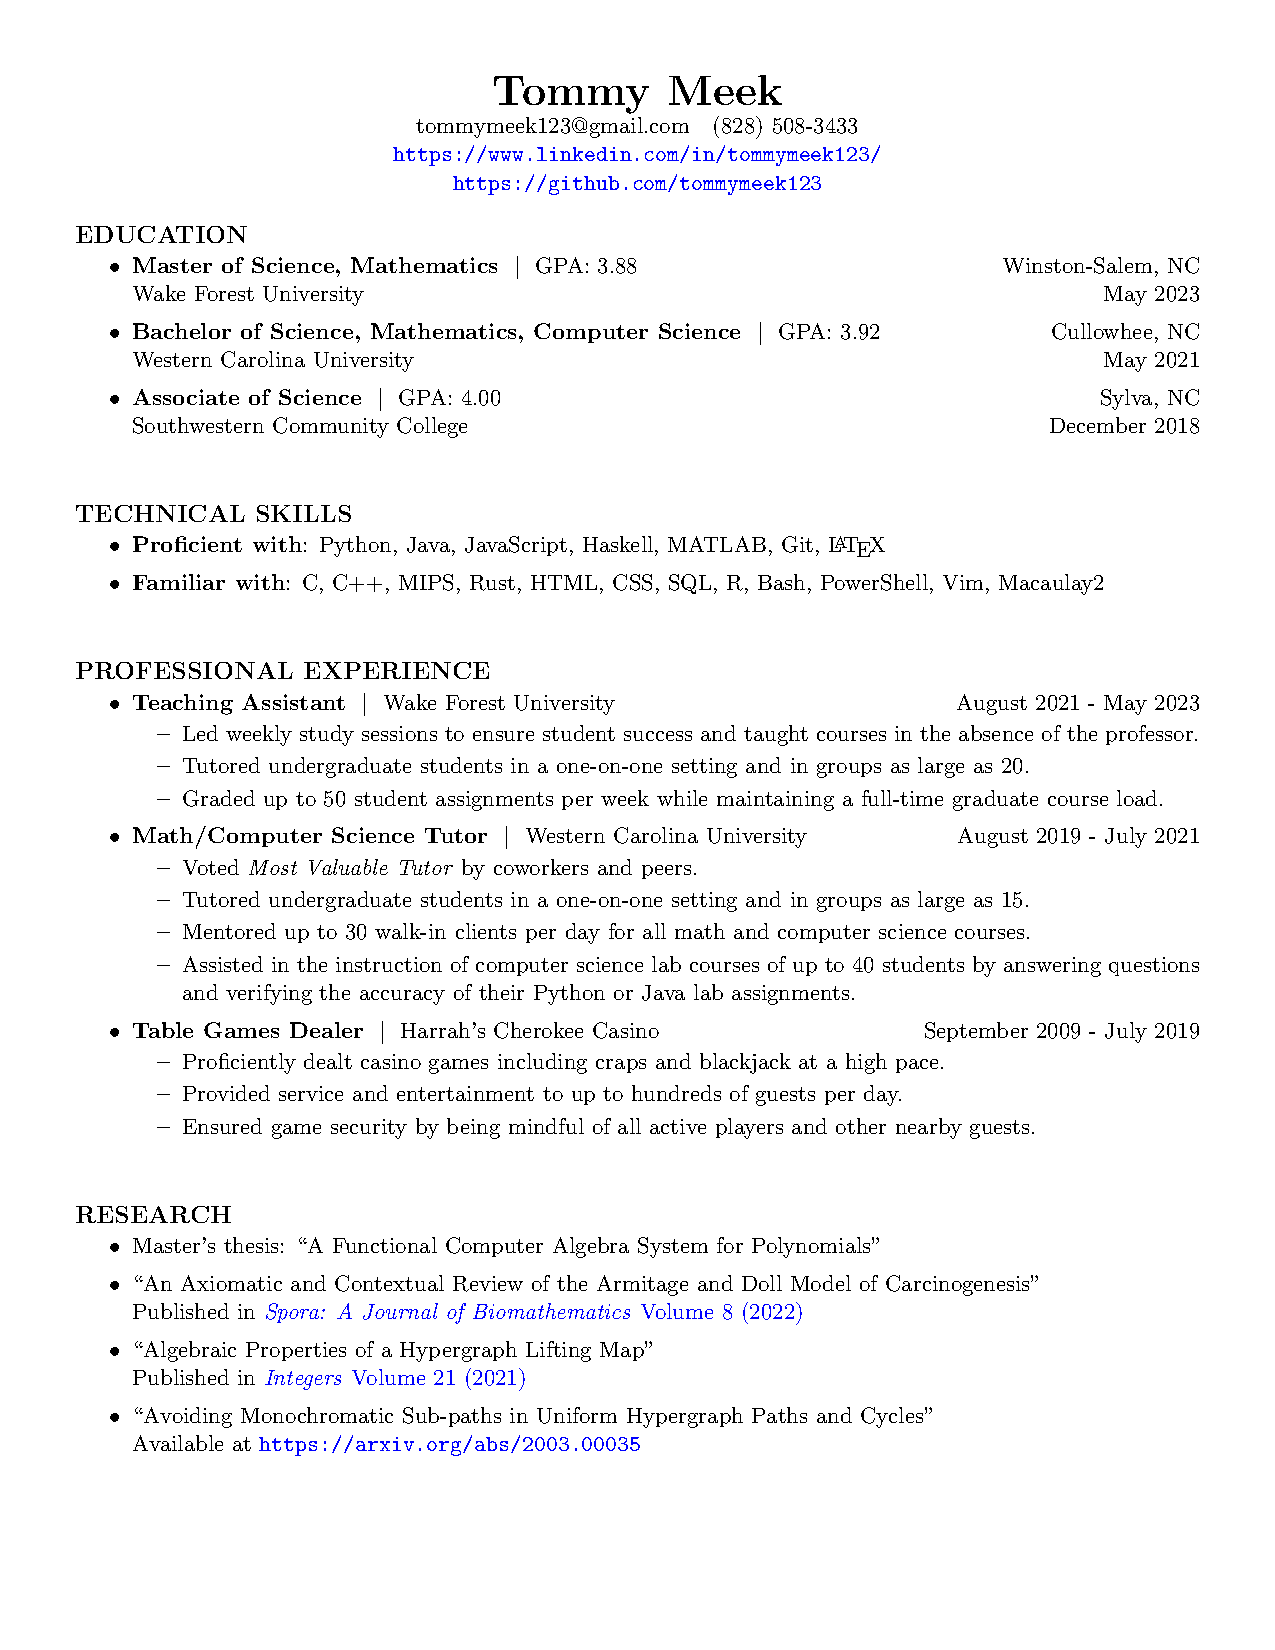
\includepdf[trim=-30mm 0mm -10mm 0mm, pages=-]{CV.pdf}

\end{document}